%%%%%%%%%%%%%%%%%%%%%%%%%%%%%%%%%%%%%%%%%%%%%%%%%%%%%%%%%%%%%%%%%%%%
%%%%%%%%%%%%%%%%%%%%%%%%%%%%%%%%%%%%%%%%%%%%%%%%%%%%%%%%%%%%%%%%%%%%
%%                                                                %%
%% An example for writting your thesis using LaTeX                %%
%% Original version by Luis Costa,  changes by Perttu Puska       %%
%% Support for Swedish added 15092014                             %%
%%                                                                %%
%% This example consists of the files                             %%
%%         thesistemplate.tex (versio 2.01)                       %%
%%         opinnaytepohja.tex (versio 2.01) (for text in Finnish) %%
%%         aaltothesis.cls (versio 2.01)                          %%
%%         kuva1.eps                                              %%
%%         kuva2.eps                                              %%
%%         kuva1.pdf                                              %%
%%         kuva2.pdf                                              %%
%%                                                                %%
%%                                                                %%
%% Typeset either with                                            %%
%% latex:                                                         %%
%%             $ latex opinnaytepohja                             %%
%%             $ latex opinnaytepohja                             %%
%%                                                                %%
%%   Result is the file opinnayte.dvi, which                      %%
%%   is converted to ps format as follows:                        %%
%%                                                                %%
%%             $ dvips opinnaytepohja -o                          %%
%%                                                                %%
%%   and then to pdf as follows:                                  %%
%%                                                                %%
%%             $ ps2pdf opinnaytepohja.ps                         %%
%%                                                                %%
%% Or                                                             %%
%% pdflatex:                                                      %%
%%             $ pdflatex opinnaytepohja                          %%
%%             $ pdflatex opinnaytepohja                          %%
%%                                                                %%
%%   Result is the file opinnaytepohja.pdf                        %%
%%                                                                %%
%% Explanatory comments in this example begin with                %%
%% the characters %%, and changes that the user can make          %%
%% with the character %                                           %%
%%                                                                %%
%%%%%%%%%%%%%%%%%%%%%%%%%%%%%%%%%%%%%%%%%%%%%%%%%%%%%%%%%%%%%%%%%%%%
%%%%%%%%%%%%%%%%%%%%%%%%%%%%%%%%%%%%%%%%%%%%%%%%%%%%%%%%%%%%%%%%%%%%

%% Uncomment one of these:
%% the 1st when using pdflatex, which directly typesets your document in
%% pdf (use jpg or pdf figures), or
%% the 2nd when producing a ps file (use eps figures, don't use ps figures!).
\documentclass[english,12pt,a4paper,pdftex,sci,utf8]{aaltothesis}
%\documentclass[english,12pt,a4paper,dvips]{aaltothesis}

%% To the \documentclass above
%% specify your school: arts, biz, chem, elec, eng, sci
%% specify the character encoding scheme used by your editor: utf8, latin1

%% Use one of these if you write in Finnish (see the Finnish template):
%%
%\documentclass[finnish,12pt,a4paper,pdftex,elec,utf8]{aaltothesis}
%\documentclass[finnish,12pt,a4paper,dvips]{aaltothesis}

\usepackage{graphicx}
\usepackage[inkscapelatex=false]{svg}
\usepackage{tikz}
\usepackage[absolute,overlay]{textpos}
\usetikzlibrary{arrows.meta, positioning}
\usepackage{caption}
\usepackage{subcaption}
\usepackage{float} % For [H]
\usepackage[ruled]{algorithm2e}
\usepackage{threeparttable}
\usepackage{booktabs}
\SetKwComment{Comment}{/* }{ */}




%% Use this if you write hard core mathematics, these are usually needed
\usepackage{amsfonts,amssymb,amsbsy, amsmath}


%% Use the macros in this package to change how the hyperref package below 
%% typesets its hypertext -- hyperlink colour, font, etc. See the package
%% documentation. It also defines the \url macro, so use the package when 
%% not using the hyperref package.
%%
%\usepackage{url}

%% Use this if you want to get links and nice output. Works well with pdflatex.
\usepackage[hidelinks]{hyperref}
\hypersetup{pdfpagemode=UseNone, pdfstartview=FitH,
  colorlinks=true,urlcolor=blue,linkcolor=blue,citecolor=black,
  pdftitle={Default Title, Modify},pdfauthor={Your Name},
  pdfkeywords={Modify keywords}}
\usepackage[capitalise,noabbrev]{cleveref}


\usepackage{float}


%% All that is printed on paper starts here
\begin{document}

%% Change the school field to specify your school if the automatically 
%% set name is wrong
 \university{aalto University}
 \school{School of Science}

%% Only for B.Sc. thesis: Choose your degree programme. 
\degreeprogram{Computer Science}
%%


%% Valitse yksi näistä kolmesta
%%
%% Choose one of these:
\univdegree{BSc}
%\univdegree{MSc}
%\univdegree{Lic}

%% Your own name (should be self explanatory...)
\author{Daniel Michaeli}

%% Your thesis title comes here and again before a possible abstract in
%% Finnish or Swedish . If the title is very long and latex does an
%% unsatisfactory job of breaking the lines, you will have to force a
%% linebreak with the \\ control character. 
%% Do not hyphenate titles.
%% 

\thesistitle{GPU-Accelerated Option Pricing Algorithms}
\place{Espoo}

%% For B.Sc. thesis use the date when you present your thesis. 
%% 
%% Kandidaatintyön päivämäärä on sen esityspäivämäärä! 
\date{16.2.2025}

%% B.Sc. or M.Sc. thesis supervisor 
%% Note the "\" after the comma. This forces the following space to be 
%% a normal interword space, not the space that starts a new sentence. 
%% This is done because the fullstop isn't the end of the sentence that
%% should be followed by a slightly longer space but is to be followed
%% by a regular space.
%%
\supervisor{M.Sc.\ Henrik Lievonen} %{Prof.\ Pirjo Professori}

%% B.Sc. or M.Sc. thesis advisors(s). You can give upto two advisors in
%% this template. Check with your supervisor how many official advisors
%% you can have.
%%
%\advisor{Prof.\ Pirjo Professori}
%\advisor{D.Sc.\ (Tech.) Olli Ohjaaja}
\advisor{M.Sc.\ Henrik Lievonen}

%% Aalto logo: syntax:
%% \uselogo{aaltoRed|aaltoBlue|aaltoYellow|aaltoGray|aaltoGrayScale}{?|!|''}
%%
%% Logo language is set to be the same as the document language.
%% Logon kieli on sama kuin dokumentin kieli
%%
\uselogo{aaltoBlack}{''}

%% Create the coverpage
%%
\makecoverpage


%% Note that when writting your master's thesis in English, place
%% the English abstract first followed by the possible Finnish abstract

%% English abstract.
%% All the information required in the abstract (your name, thesis title, etc.)
%% is used as specified above.
%% Specify keywords
%%
%% Kaikki tiivistelmässä tarvittava tieto (nimesi, työnnimi, jne.) käytetään
%% niin kuin se on yllä määritelty.
%% Avainsanat
%%
\keywords{moi, mojn, moin, morjens, moro}
%% Abstract text
\begin{abstractpage}[english]

English bla bla bla
\end{abstractpage}

%% Force a new page so that the possible English abstract starts on a new page
%%
%% Pakotetaan uusi sivu varmuuden vuoksi, jotta 
%% mahdollinen suomenkielinen ja englanninkielinen tiivistelmä
%% eivät tule vahingossakaan samalle sivulle
\newpage
%

%% Force new page so that the Swedish abstract starts from a new page
\newpage
%
%% Swedish abstract. Delete if you don't need it. 
%% 
\thesistitle{Genomströmning och latens i datorsystem: en anlays av avvägningseffekter och optimeringsstrategier}
\advisor{M.Sc.\ Henrik Lievonen} %
\degreeprogram{Datateknik}
\department{Högskolan för teknikvetenskaper}%
\professorship{?}  %
%% Abstract keywords
\keywords{Nyckelord p\aa{} svenska,\\ Moi, moin, moidå, mojjdå}
%% Abstract text
\begin{abstractpage}[swedish]
 svenska bla bla bla
\end{abstractpage}

\newpage


%% Table of contents. 

\thesistableofcontents




%% Tweaks the page numbering to meet the requirement of the thesis format:
%% Begin the pagenumbering in Arabian numerals (and leave the first page
%% of the text body empty, see \thispagestyle{empty} below).
%% Additionally, force the actual text to begin on a new page with the 
%% \clearpage command.
%% \clearpage is similar to \newpage, but it also flushes the floats (figures
%% and tables).
%% There is no need to change these
%%
\cleardoublepage
\storeinipagenumber
\pagenumbering{arabic}
\setcounter{page}{1}


%% Text body begins. Note that since the text body
%% is mostly in Finnish the majority of comments are
%% also in Finnish after this point. There is no point in explaining
%% Finnish-language specific thesis conventions in English. Someday 
%% this text will possibly be translated to English.
%%
\section{Introduction}
%% Leave first page empty
\thispagestyle{empty}
Options are financial contracts between two parties that grant the holder the right, but not the obligation, to buy or sell an underlying asset at a predetermined price by a future date \cite{hull2016options}. Options belong to a broader class of financial instruments known as derivatives, which derive their value from the price of the underlying asset. These instruments enable both speculative trading and risk management strategies, making them attractive even to non-financial institutions \cite{bartram2009international}. The derivatives market has experienced substantial growth over the past half-century, driven by advances in financial mathematics \cite{merton1994influence} and exponential increases in affordable computing power \cite{nordhaus2007two}.

Modern option pricing employs various models with different theoretical foundations and computational requirements. Execution speed is often critical. For example, high-frequency trading strategies exploit transient pricing anomalies through millions of rapid transactions, where millisecond delays can determine profitability. Faster computation also benefits risk management practices that rely on extensive portfolio simulations across multiple market scenarios. These performance requirements have motivated research into adapting option pricing algorithms to leverage the GPU's parallel computing capabilities.

This thesis reviews GPU acceleration of common option pricing algorithms. The objectives are to assess how algorithm dependency structures affect parallelization potential, determine which algorithms achieve the greatest performance improvements, and identify bottlenecks. The analysis considers the Cox-Ross-Rubinstein (CRR) binomial model and Monte Carlo (MC) methods for option pricing. The Black-Scholes-Merton (BSM) model is omitted as it is an analytical formula rather than an algorithm, providing no meaningful parallelization opportunities beyond arithmetic operations. PDE-based numerical methods, while offering substantial parallelization challenges, require mathematical foundations beyond the scope of this thesis.

~\cref{sec:theory} establishes formal definitions and fundamental option pricing theory. ~\cref{sec:gpu} examines GPU architecture and introduces parallel computing concepts for algorithm analysis. ~\cref{sec:gpu-crr} and~\cref{sec:gpu-mc} analyze GPU implementations of the CRR and MC algorithms, respectively. ~\cref{sec:summary-conclusions} summarizes the findings and presents conclusions.

For scope restriction purposes, the following choices have been made:
\begin{itemize}\setlength\itemsep{0.1em}
\item The analysis focuses mainly on European and American options, collectively termed \emph{vanilla options}, with the exception of Monte Carlo methods that naturally handle \emph{exotic options} with complex payoff structures. All underlying assets are assumed to be non-dividend-paying.
    
\item The implementations are evaluated solely on computational performance --- specifically execution time and parallelization efficiency. Accuracy, numerical stability, and other properties are not considered.

\item The reviewed research uses varying architectures, optimization levels, and performance metrics, making direct quantitative comparison infeasible. \mbox{Analysis} therefore focuses on relative speedups of GPU implementations over baselines.
\end{itemize}

%% In a thesis, every section starts a new page, hence \clearpage
\clearpage

\section{Fundamentals of Option Pricing} \label{sec:theory}

The following section provides the theoretical background necessary to understand option pricing and the algorithms that will be GPU-accelerated. First, general definitions are established along with vanilla option payoffs. The section then covers the key determinants of option prices. Two essential principles anchor the theoretical framework: \emph{no-arbitrage pricing} and \emph{risk-neutral valuation}. Together, these concepts form the mathematical foundation underlying modern option pricing models.

\subsection{Definitions}\label{subsec:definitions}
The following terminology is adapted from Hull's ``Options, Futures, and Other Derivatives'' \cite{hull2016options}:

\vspace{0.5\baselineskip}
\noindent\textbf{Call Option.} A contract granting the holder the right, but not the obligation, to purchase an underlying asset at a predetermined price by a specified date.

\vspace{0.5\baselineskip}
\noindent\textbf{Put Option.} A contract granting the holder the right, but not the obligation, to sell an underlying asset at a predetermined price by a specified date.

\vspace{0.5\baselineskip}
\noindent\textbf{Strike Price.} The predetermined price at which the underlying asset may be bought (call) or sold (put) when the option is exercised.

\vspace{0.5\baselineskip}
\noindent\textbf{Maturity.} The expiration date of the option contract, after which it becomes worthless if not exercised.

\vspace{\baselineskip}
\noindent The phrase ``by a specified date'' warrants clarification, as exercise rules vary by option style. \emph{European options} may be exercised only at maturity, while \emph{American options} can be exercised at any time before maturity. Throughout this thesis, the underlying asset is generally referred to as ``the stock,'' with its current market value denoted as the \emph{spot price}.

Every option contract involves two parties with opposing positions. The buyer assumes the \emph{long position}, paying an upfront premium for the right to exercise the option. The seller --- also known as the option writer --- takes the corresponding \emph{short position}, receiving the premium in exchange for accepting the obligation to fulfill the contract if exercised.

\clearpage
\subsection{Vanilla Option Payoffs}\label{subsec:payoffs}

Options are zero-sum contracts: gains to one party exactly offset losses to the other. The \emph{payoff} of an option represents its intrinsic value at exercise, whereas the profit accounts for the premium paid or received: \mbox{$\text{profit} = \text{payoff} - \text{premium}$} for long positions. The payoff is mechanically determined by the option's characteristics and market conditions at exercise, while the premium is the upfront cost determined by market participants. Option pricing models aim to determine the theoretical fair value of this premium.

The following presentation of option payoffs draws from Hull \cite{hull2016options} and Hull et al. \cite{hull2013fundamentals}. It presents diagrams that visualize how profit varies with the spot price at exercise. Each vanilla option type is examined through both long and short positions, supplemented by practical examples. For simplicity, all options are written on one share of the underlying stock, transaction costs and taxes are ignored, and markets are assumed sufficiently liquid to permit instantaneous trading.

A call option buyer pays a premium upfront to secure the right to purchase stock at the strike price. This position profits when the stock price rises sufficiently to offset the premium paid. Figure~\ref{fig:long_call_payoff} illustrates this long position. Let $S_T$ denote the spot price at exercise and $K$ the strike price. When $S_T < K$, the option is said to be \emph{out of the money (OTM)} and has zero payoff. At $S_T = K$, the option is \emph{at the money (ATM)}, and when $S_T > K$, the option becomes \emph{in the money (ITM)} with payoff $S_T - K$ \cite{hull2013fundamentals}. However, the position only becomes profitable once the payoff offsets the premium paid. The ``moneyness'' terminology always reflects the perspective of the long position. Rational investors exercise ITM options to capture the payoff, even if it only partially offsets the premium paid. In liquid markets, this involves buying stock at the strike price and immediately selling at the higher spot price.

To demonstrate the use of options for risk management, consider a manufacturer dependent on crude oil who anticipates price increases. By purchasing call options, they fix a price ceiling for future oil purchases, effectively buying insurance against adverse price movements. The premium represents the cost of this protection, with the strike price chosen to align with their risk tolerance and budget constraints.

\begin{center}
\begin{figure}[H]
\centering
    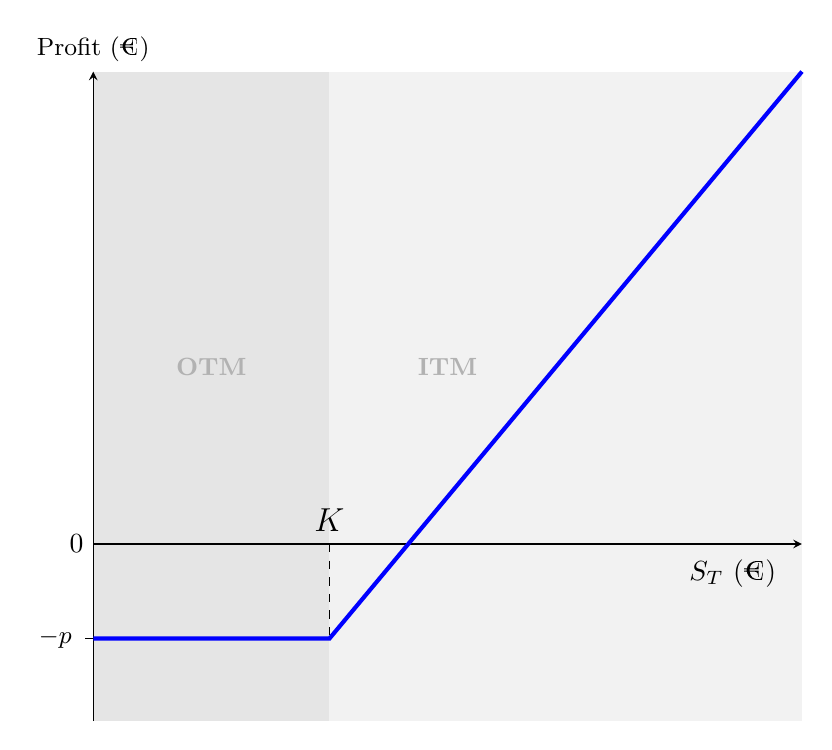
\begin{tikzpicture}[scale=1.5, >=stealth]
        \fill[gray!10] (2,-1.5) -- (6,-1.5) -- (6,4) -- (2,4) -- cycle;
        \fill[gray!20] (0,-1.5) -- (2,-1.5) -- (2,4) -- (0,4) -- cycle;
        \draw[->] (0,0) -- (6,0) node[below,xshift=-25,yshift=-2pt, align=center] {$S_T$ (€)};
        \draw[->] (0,-1.5) -- (0,4) node[above] {\small Profit (€)};
        \draw[dashed] (2,0) -- (2,-0.8) node[above, yshift=35] {\large$K$};
        \draw[line width=1.5pt, blue] (0,-0.8) -- (2,-0.8) -- (6,4);
        \node[left] at (0,0) {0};
        \draw (-0.07,-0.8) -- (0,-0.8);
        \node[left] at (-0.1,-0.8) {\small $-p$};
        \node[gray!60] at (3,1.5) {\small \textbf{ITM}};
        \node[gray!60] at (1,1.5) {\small \textbf{OTM}};
    \end{tikzpicture}
    \caption{Profit diagram for the long position in a call option. $K$ = strike price, \mbox{$S_T$ = spot price} at exercise, $p$ = premium. The buyer pays a premium to secure the right to purchase stock at price $K$. When $S_T < K$, the option is out of the money (OTM) and expires worthless with profit $-p$. When $S_T > K$, the option is in the money (ITM) and is exercised: the buyer purchases stock for $K$ to sell at $S_T$. The position becomes profitable only when $S_T - K > p$.}
    \label{fig:long_call_payoff}
\end{figure}
\end{center}

The short call position has an inverse profit diagram. When the option is OTM, it expires worthless and the writer retains the full premium as profit. When it is ITM, the buyer exercises, forcing the writer to sell the stock at the strike price $K$ despite the higher spot price $S_T$ \cite{hull2013fundamentals}. The position remains profitable as long as the premium offsets this loss, with break-even at $S_T - K = p$. ~\cref{fig:short_call_payoff} illustrates the corresponding profit diagram. Continuing with the previous example, this position could be taken by a crude oil producer expecting prices to remain below or near the strike price at maturity. The risk taken by the writer commands the premium.

The payoff from the long position in a call option is defined as
\begin{equation}
    \max(S_T-K,0)
\label{eq:long_call_payoff}
\end{equation}
as the buyer will only exercise when ITM to either profit or offset losses. Consequently, the payoff from the short position is defined as 
\begin{equation*}
    -\max(S_T-K,0) = \min(K-S_T,0)
\end{equation*}
due to the zero-sum nature of the contract \cite{hull2016options}.\footnote{For American options with the right to early-exercise, the payoff is calculated using $S_\tau$ instead of $S_T$, where $\tau \le T$ is the chosen point of exercise.}

\begin{center}
\begin{figure}[H]
\centering
    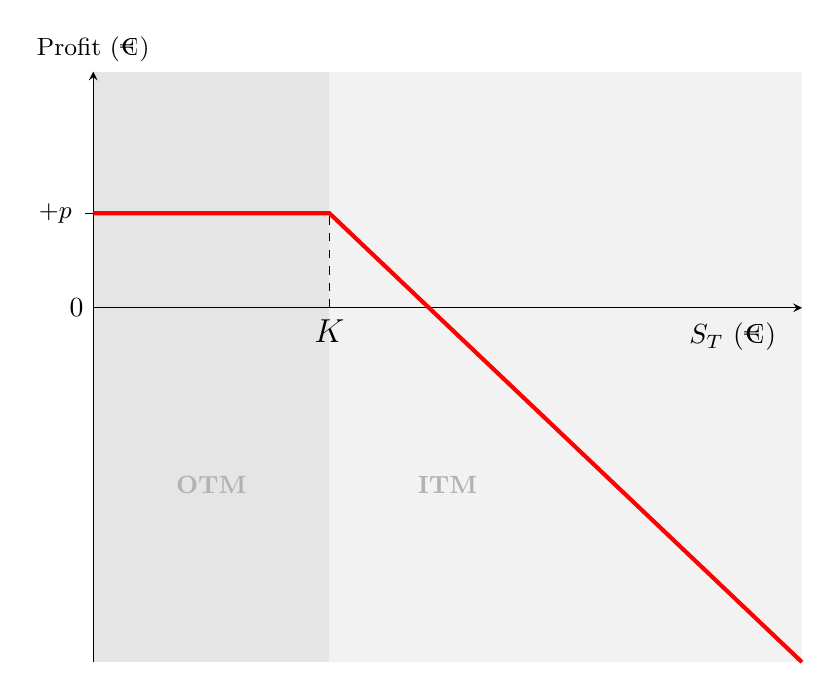
\begin{tikzpicture}[scale=1.5, >=stealth]
        \fill[gray!10] (2,-3) -- (6,-3) -- (6,2) -- (2,2) -- cycle;
        \fill[gray!20] (0,-3) -- (2,-3) -- (2,2) -- (0,2) -- cycle;
        \draw[->] (0,0) -- (6,0) node[below,xshift=-25,yshift=-2pt, align=center] {$S_T$ (€)};
        \draw[->] (0,-3) -- (0,2) node[above] {\small Profit (€)};
        \draw[dashed] (2,0) -- (2,0.8) node[below, yshift=-35] {\large$K$};
        \draw[line width=1.5pt, red] (0,0.8) -- (2,0.8) -- (6,-3);
        \node[left] at (0,0) {0};
        \draw (-0.07,0.8) -- (0,0.8);
        \node[left] at (-0.1,0.8) {\small $+p$};
        \node[gray!60] at (1,-1.5) {\small \textbf{OTM}};
        \node[gray!60] at (3,-1.5) {\small \textbf{ITM}};
    \end{tikzpicture}
    \caption{Profit diagram for the short position in a call option. $K$ = strike price, $S_T$ = spot price at exercise, $p$ = premium. The writer receives a premium for the obligation to sell stock at price $K$. When $S_T < K$, the option is out of the money (OTM) and expires worthless. As it is not exercised, the writer retains the full premium $p$ as profit. When $S_T > K$, the option is in the money (ITM) and is exercised: the writer is forced to sell the stock at the strike price $K$ despite the higher spot price $S_T$. The profit decreases linearly with $S_T$, becoming negative once $S_T - K > p$.}
    \label{fig:short_call_payoff}
\end{figure}
\end{center}

A put option buyer pays a premium upfront to secure the right to sell stock at the strike price. This position profits when the stock price falls sufficiently to offset the premium paid. Figure~\ref{fig:put_option_payoffs} illustrates both long and short positions. When $S_T > K$, the put option is OTM and expires worthless --- no rational investor would sell at the strike price $K$ when they could sell at the higher spot price $S_T$. When $S_T < K$, the option becomes ITM with payoff $K - S_T$ \cite{hull2013fundamentals}. The buyer profits only when this payoff exceeds the premium paid. At exercise, the buyer can buy stock at the spot price and immediately sell it at the higher strike price.

The short put position profits under opposite conditions. When the option is OTM, it expires worthless and the writer retains the full premium as profit. When it is ITM, the buyer exercises, forcing the writer to purchase stock at the strike price $K$ despite the lower spot price $S_T$ \cite{hull2013fundamentals}. The position remains profitable as long as the premium offsets this loss, with break-even at $K - S_T = p$.

An example use case would be a crude oil supplier forecasting low prices in a year's time and taking the long position to secure a minimum revenue. A premium is paid to hedge against unfavorable price movements. The short position would be taken by a market participant who anticipates crude oil prices not to fall enough to offset the premium.


\begin{figure}[H]
\centering

\begin{subfigure}[t]{0.45\textwidth}
\centering
\resizebox{\linewidth}{!}{%
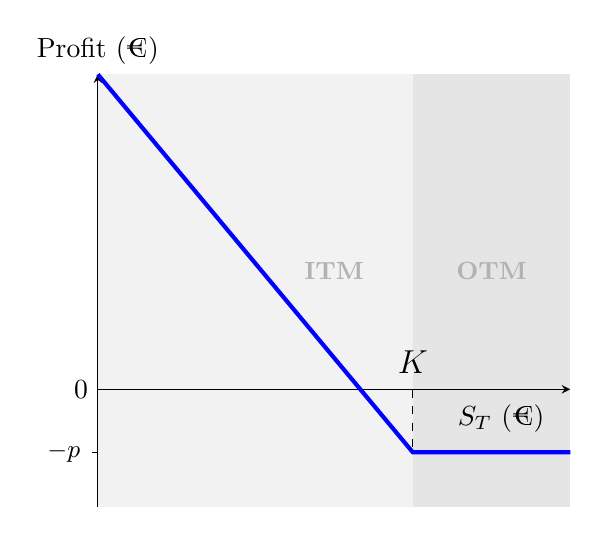
\begin{tikzpicture}[>=stealth]
    \fill[gray!20] (4,-1.5) -- (6,-1.5) -- (6,4) -- (4,4) -- cycle;
    \fill[gray!10] (0,-1.5) -- (4,-1.5) -- (4,4) -- (0,4) -- cycle;
    \draw[->] (0,0) -- (6,0) node[below,xshift=-25,yshift=-2pt] {$S_T$ (€)};
    \draw[->] (0,-1.5) -- (0,4) node[above] {Profit (€)};
    \draw[dashed] (4,0) -- (4,-0.8) node[above,yshift=25] {\large$K$};
    \draw[line width=1.5pt, blue] (0,4) -- (4,-0.8) -- (6,-0.8);
    \node[left] at (0,0) {0};
    \draw (-0.07,-0.8) -- (0,-0.8);
    \node[left] at (-0.1,-0.8) {\small $-p$};
    \node[gray!60] at (3,1.5) {\small \textbf{ITM}};
    \node[gray!60] at (5,1.5) {\small \textbf{OTM}};
\end{tikzpicture}%
}
\caption{Long put position}
\end{subfigure}
\hfill
\begin{subfigure}[t]{0.45\textwidth}
\centering
\resizebox{\linewidth}{!}{%
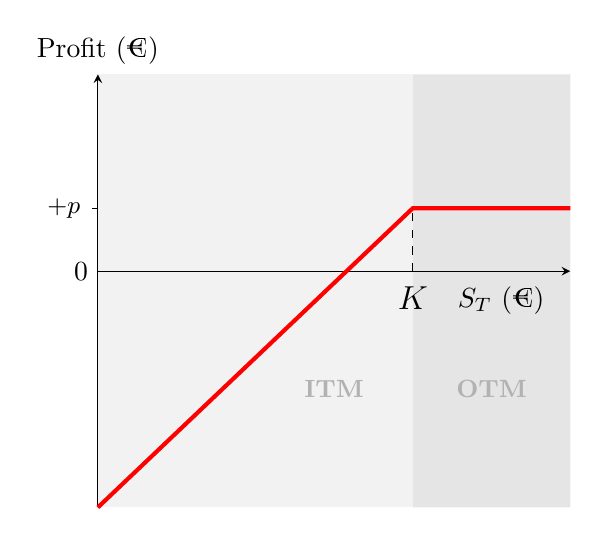
\begin{tikzpicture}[>=stealth]
    \fill[gray!20] (4,-3) -- (6,-3) -- (6,2.5) -- (2,2.5) -- cycle;
    \fill[gray!10] (0,-3) -- (4,-3) -- (4,2.5) -- (0,2.5) -- cycle;
    \draw[->] (0,0) -- (6,0) node[below,xshift=-25,yshift=-2pt] {$S_T$ (€)};
    \draw[->] (0,-3) -- (0,2.5) node[above] {Profit (€)};
    \draw[dashed] (4,0) -- (4,0.8) node[below,yshift=-25] {\large$K$};
    \draw[line width=1.5pt, red] (0,-3) -- (4,0.8) -- (6,0.8);
    \node[left] at (0,0) {0};
    \draw (-0.07,0.8) -- (0,0.8);
    \node[left] at (-0.1,0.8) {\small $+p$};
    \node[gray!60] at (5,-1.5) {\small \textbf{OTM}};
    \node[gray!60] at (3,-1.5) {\small \textbf{ITM}};
\end{tikzpicture}%
}
\caption{Short put position}
\end{subfigure}
\caption{Profit diagrams for long (a) and short (b) positions in a put option. \mbox{$K$ = strike price}, $S_T$ = spot price at exercise, $p$ = premium. (a) The buyer pays the premium $p$ for the right to sell stock at strike price $K$. When $S_T < K$, the option is in the money (ITM) and is exercised. The position profits when $K - S_T > p$. When $S_T > K$, the option is out of the money (OTM) and expires worthless with \mbox{loss $-p$}. (b) The writer receives premium $p$ for the obligation to buy at price $K$. When ITM, the writer must purchase at the strike price $K$ despite the lower spot price $S_T$. When OTM, the option expires worthless and the writer keeps the premium $p$. The position becomes unprofitable when $K - S_T > p$.}
\label{fig:put_option_payoffs}
\end{figure}

The payoff from the long position in a put option is defined as
\begin{equation}
    \max(K-S_T,0)
\label{eq:long_put_payoff}
\end{equation}
as being ITM now means $K > S_T$ \cite{hull2016options}. Conversely, the payoff in the corresponding short position is defined as
\begin{equation*}
    -\max(K-S_T,0) = \min(S_T-K,0).
\end{equation*}
The buyer of an option is never obligated to exercise, and the loss is therefore limited to the premium paid. On the other hand, the writer is always obligated to potentially engage in a disadvantageous trade with the buyer. Additionally, since underlying asset prices have no theoretical upper bound but are limited to non-negative values, the short call position faces potentially unlimited losses. \cref{tab:options_table} aggregates information about the extreme-case profit and loss incurred from the different option types and positions.

\begin{table}[!htb]
\centering
\caption{Extreme-case upside and downside potential for different option positions. \mbox{$p$ = premium}, $K$ = strike price. The long position in a call option has unlimited upside potential due to theoretically unbounded underlying asset prices, with losses limited to the premium paid. The corresponding short position inverts this behavior with unlimited downside risk. Put options have bounded payoffs as asset prices cannot fall below zero. The maximum gain for a long put position is $K-p$ when the spot price reaches zero, and the maximum loss for the corresponding short position is $-(K-p)$.}\label{tab:options_table}
\begin{tabular}{|l|p{5cm}|p{5cm}|}
\hline
\textbf{} & \textbf{Call Option} & \textbf{Put Option} \\
\hline
\textbf{Long} & \textbf{Maximum Gain:} $+\infty$
\newline \textbf{Maximum Loss:} $-p$ & \textbf{Maximum Gain:} $K-p$
\newline \textbf{Maximum Loss:} $-p$ \\
\hline
\textbf{Short} & \textbf{Maximum Gain:} $+p$
\newline \textbf{Maximum Loss:} $-\infty$ & \textbf{Maximum Gain:} $+p$
\newline \textbf{Maximum Loss:} $-(K-p)$ \\
\hline
\end{tabular}
\end{table}
Pricing models aim to determine the theoretical fair value of the option \mbox{premium $p$.} While market prices form through supply and demand dynamics, they remain anchored by mathematical and economic principles. Short-term deviations occur, but prices tend to converge toward theoretically justified values over time as mispricing creates correcting trading opportunities.
\clearpage

\subsection{Price Determinants}

Hull et al.\ \cite{hull2013fundamentals} define the following primary factors that affect an option's value. While these serve as parameters in pricing models, their directional effects can be reasoned through without formal mathematics. The analysis examines each factor in isolation (ceteris paribus), although they often interact with each other in practice.

\paragraph{Stock Price.} The relationship between stock and option prices follows directly from the payoff definitions. Call option values increase with stock price, while put option values decrease, as demonstrated in \cref{subsec:payoffs}.

\paragraph{Volatility.} Higher volatility increases both call and put option values. The asymmetric risk-reward profile --- losses limited to premium paid versus potentially large gains --- means increased price variability improves expected outcomes. This effect is most pronounced for OTM options that require significant price movements to gain value.

\paragraph{Maturity.} Following the asymmetric risk-reward logic, longer-dated options generally command higher premiums due to increased opportunity for favorable price movements. American options particularly benefit through early-exercise flexibility. However, expected dividends can reverse this relationship for call options --- an option expiring before the ex-dividend date may be worth more than one expiring after, since dividends reduce stock prices without benefiting option holders \cite{hull2013fundamentals}.

\paragraph{Risk-Free Rate.} The risk-free rate represents the return on a theoretically risk-free investment, such as a government bond, and serves as a baseline for valuing riskier assets. In option pricing, it affects value by discounting future cash flows. Higher interest rates reduce the present value of the strike price. For call options, this makes exercising cheaper in present terms, increasing the option’s value. For puts, it reduces the value of the payoff received, lowering the option’s price. In real markets, interest rate changes also influence stock prices, complicating this relationship.

\paragraph{Dividends.} Expected dividend payments decrease the value of calls and increase the value of puts, as stock prices typically drop on ex-dividend dates without benefiting option holders. This effect is most significant for longer-dated options that span multiple dividend payments.
\clearpage


\subsection{No-Arbitrage Pricing and Risk-Neutral Valuation}\label{sec:risk-neutral-theory}

This section introduces ideas from the work of Fischer Black, Myron Scholes, and Robert Merton that revolutionized option pricing and led to the 1997 Nobel Prize in Economic Sciences\footnote{The prize was awarded to Scholes and Merton; Black had passed away in 1995.}. Their breakthrough insight was showing how a portfolio could be constructed to replicate and thus price an option. This replicating portfolio approach, and its elegant reformulation using risk-neutral probabilities, form the foundation for all modern option pricing models, including the CRR binomial model and MC methods. The presentation emphasizes intuition over rigor, and avid readers are encouraged to explore the references in greater detail \cite{hull2016options, gisiger2010risk, tham2001risk}. The assumptions presented in \cref{subsec:payoffs} continue to hold.

Traditional asset valuation discounts expected future cash flows to present value. For options, this approach faced fundamental problems: calculating the expected payoff required assigning probabilities to future stock prices --- an inherently difficult and at least partially subjective task. Even if the expected payoff were somehow known, there was no consistent way to determine the appropriate discount rate, as investors naturally have differing risk preferences \cite{nobel1997}. The key insight was recognizing that these subjective estimates could be circumvented entirely by making a reasonable assumption about market behavior --- the absence of arbitrage.

\emph{Arbitrage} denotes simultaneous buying and selling of an asset at different prices to make risk-free profit. Imagine tomato prices being lower in town A than town B due to an exceptionally good harvest. An astute tradesman could buy tomatoes in town A and immediately sell them in town B, pocketing the difference without taking any position on future price movements. This opportunity is self-eliminating: as the tradesman introduces more tomatoes from town A into town B, the corresponding prices adjust to the changes in supply until an equilibrium is reached \cite{hull2016options, wilmott2013paul}. Other traders observing this opportunity might adopt the same strategy, eliminating it even faster. While arbitrage opportunities do arise, they are typically rare and short-lived in modern markets, as sophisticated traders quickly eliminate them. Hence, the no-arbitrage assumption is reasonable, at least over longer time periods.

It logically follows that in absence of arbitrage opportunities, two assets producing identical cash flows must be equally valued \cite{hull2016options, wilmott2013paul}. This conclusion suggests a new approach: construct a portfolio that matches the option payoff in all scenarios. The option value must then equal the price of constructing such a portfolio.

Hull~et~al.~\cite{hull2013fundamentals} demonstrate this approach using a one-period binomial model. The current stock price $S_0$ can move to either $S_0u$ or $S_0d$ ($u>1,d<1$) after time~$T$. These prices result in option payoffs $f_u$ and $f_d$ respectively. \cref{fig:oneperiodbinom} illustrates the setup. Restricting the stock price to two future outcomes makes it possible to construct a \emph{replicating portfolio}, consisting of $\Delta$ shares of the stock and $B$ amount of a risk-free asset growing at the risk-free rate $r$. Equating the portfolio value with the option payoff in each future state gives:

\begin{equation*}
\begin{cases}
    \Delta (S_0u) + B(1+r) = f_u\\
    \Delta (S_0d) + B(1+r) = f_d
\end{cases}.
\end{equation*}
Solving for $\Delta$ and $B$ yields
\begin{equation*}
\begin{cases}
    \Delta = \frac{f_u - f_d}{S_0(u-d)}\\
    B = \frac{f_du-f_ud}{(u-d)(1+r)}
\end{cases}.
\end{equation*}
It is evidently possible to construct a portfolio with identical payoff as the option itself, according to
\begin{equation}
     \frac{f_u - f_d}{S_0(u-d)} S_0 + \frac{f_du-f_ud}{(u-d)(1+r)}
\label{eq:replicating-portfolio}.
\end{equation}
Under the no-arbitrage assumption, the value of the option must equal the price of constructing this portfolio, that is buying $\Delta$ shares and investing $B$ in a risk-free asset. A negative $\Delta$ implies shorting the stock\footnote{Short selling involves borrowing shares from a broker, selling them immediately at the current price, and later repurchasing them to return to the lender. If the price falls, the short seller profits from the difference.}, and a negative $B$ implies borrowing money at the risk-free rate instead of investing it.
\begin{figure}[htbp]
    \centering
    \begin{tikzpicture}[
        scale=1.5,
        >=stealth,
        every node/.style={font=\normalsize}
    ]
    \node (S0) at (0,0) {$S_0$};
    \node (Su) at (4,2) {$S_0u$};
    \node (Sd) at (4,-2) {$S_0d$};
    \node at (0,-0.5) {$f$};
    \node at (4,1.5) {$f_u$};
    \node at (4,-2.5) {$f_d$};
    \draw[->, thick] (S0) -- (Su);
    \draw[->, thick] (S0) -- (Sd);
    \draw[->, thick] (0,-3) -- (4,-3);
    \node at (0,-3) [below] {$t=0$};
    \node at (4,-3) [below] {$t=T$};
    \end{tikzpicture}
    \caption{One-period binomial model. The stock price moves from $S_0$ to either $S_0u$ or $S_0d$ over time $T$, with corresponding option values $f$, $f_u$ and $f_d$.}
    \label{fig:oneperiodbinom}
\end{figure}
The derivation assumed neither a call nor a put option, and therefore works as a pricing model for any European (and in a one-period setting, American) option. An interesting observation is that the approach utilized no information about the expected return of the stock, or the probability of its price movements. The authors motivate this intuitively by the fact that such expectations are already reflected in the stock price itself, and need not be explicitly accounted for when pricing the derivative. The option is priced relative to the underlying stock \cite{hull2016options}.\clearpage

\cref{eq:replicating-portfolio} can be rewritten as
\begin{equation*}
     \frac{1}{1+r}\left(f_u\frac{(1+r)-d}{u-d}+f_d\frac{u-(1+r)}{u-d}\right).
\end{equation*}
Defining $\tilde{p} := \frac{(1+r)-d}{u-d}$, this weight and its complement $1-\tilde{p} = \frac{u-(1+r)}{u-d}$ sum to one and lie in $[0,1]$ under the no-arbitrage condition $d \leq 1+r \leq u$, thus behaving like probabilities. The calculation can therefore be interpreted as an expected value of the option payoff, discounted at the risk-free rate:
\begin{equation}
     \frac{1}{1+r}(f_u\cdot \tilde p + f_d \cdot (1-\tilde p)).
\label{eq:risk-neutral-expectancy}
\end{equation}
While risk-neutral probabilities often cause confusion, they can simply be understood as a mathematical reformulation into a more familiar approach for pricing assets~--- discounting future cash flows. They do not reflect actual stock price movements, but rather form an artificial probability measure that yields the same price as the replicating portfolio. The term risk-neutral stems from the fact that the risk-free rate is used for discounting, resembling how a risk-neutral investor would not demand a premium for uncertain cash flows. This elegant reformulation enables tools from probability theory, and elements of it will be found in all of the models to be introduced later. Gisiger \cite{gisiger2010risk} and Tham \cite{tham2001risk} provide more formal explanations of risk-neutral valuation. The full derivation of \cref{eq:risk-neutral-expectancy} is provided in \cref{appendix:risk_neutral_derivation}.

\clearpage

\section{GPU and Parallel Computing}\label{sec:gpu}

The graphics processing unit (GPU) is a specialized processor originally designed to accelerate the rendering of images and video. The rapid growth of video games and graphics-intensive applications in the 1980s created unprecedented demand for capable hardware ~\cite{sanders2010cuda, kirk2016programming}. Graphics-related tasks like shading, rasterization, and texture mapping require massive amounts of floating-point operations per second (FLOPS), far exceeding what general-purpose CPUs could deliver. Companies like NVIDIA and ATI Technologies (later acquired by AMD) emerged as front-runners in the GPU industry \cite{sanders2010cuda}.

\emph{Latency} denotes the time between the start and completion of a single event, while \emph{throughput} measures the total amount of work performed in a given time \cite{hennessy2011computer}. These fundamental metrics are widely used to measure computing performance. Hennessy and Patterson \cite{hennessy2011computer} demonstrate that while both CPUs and GPUs have improved in both dimensions, throughput improvements have significantly outpaced latency improvements. This disparity reflects fundamental constraints: throughput can be increased by adding more processing units. Reducing latency, however, requires making individual processing units faster, which is approaching theoretical limits imposed by the laws of physics \cite{hennessy2011computer, sanders2010cuda}. Suomela's analysis of clock speed and instruction latency trends corroborate these observations \cite{suomela_ppc}. This, along with the parallel nature of graphics-related computation, led to the exceptionally throughput-optimized GPU architectures of today.

As GPU architectures evolved, researchers and developers increasingly sought to utilize their parallel computing power for non-graphics applications. However, early GPUs were not designed for general-purpose computing. The hardware lacked flexibility, and no suitable programming tools existed. Developers were forced to mask their problems as graphics operations \cite{sanders2010cuda, kirk2016programming}. This changed in 2007 when NVIDIA released CUDA (Compute Unified Device Architecture), a software abstraction layer that exposed GPU hardware capabilities through familiar C/C++ extensions. Developers could now write parallel programs directly without disguising them as pixel operations. Today, general-purpose GPU (GPGPU) applications span diverse fields, including computational finance \cite{sanders2010cuda, kirk2016programming}.
\clearpage

\subsection{CPU and GPU Architecture}
 \cref{fig:cpu-gpu-architecture} presents a simple architectural diagram of a modern CPU and GPU. The CPU diagram is based on the writings of Stallings~\cite{stallings2011operating}, while the GPU diagram is derived from both the work of Kirk and Hwu~\cite{kirk2016programming} and the CUDA C++ Programming Guide by NVIDIA~\cite{cuda2025guide}.

The CPU contains several key components working together. The arithmetic logic unit (ALU) is responsible for performing computational operations on data. Registers (not visible in the figure) store instructions, data, and memory addresses. Additional control units manage program flow and coordination with external components. The CPU executes programs in a two-step fetch-execute cycle. First, an instruction is fetched from memory and loaded into a register. The instruction is then executed, which in practice means either data processing, data transfer, or control flow operations. This cycle repeats until the program terminates, either by completing successfully, encountering an error, or being interrupted by another component.

CPUs have evolved to leverage multiple forms of parallelism. Instruction-level parallelism refers to a set of techniques to improve performance by executing multiple independent instructions simultaneously or in overlapping stages \cite{hennessy2011computer, suomela_ppc}. These techniques range from instruction pipelining and superscalar execution, which process multiple instructions concurrently, to out-of-order execution and branch prediction, which maximize pipeline utilization and anticipate control flow.

Modern CPUs also incorporate \emph{single instruction multiple data} (SIMD) capabilities through vector registers that store multiple data elements of the same type. This allows for executing a single instruction on all elements in the register simultaneously. Furthermore, most modern processors are multi-core, containing multiple instances of the core computational components. This enables thread-level parallelism, where a \emph{thread} --- an independent sequence of instructions that can be scheduled and \mbox{executed \cite{stallings2011operating}} --- can run on each core simultaneously \cite{hennessy2011computer, suomela_ppc}. Nonetheless, CPUs remain fundamentally optimized for low-latency sequential execution and control flow rather than maximizing throughput \cite{hennessy2011computer, suomela_ppc}.

\begin{figure}[htbp]
  \centering
  \begin{tikzpicture}
    \node[anchor=south west, inner sep=0] (image) at (0,0) {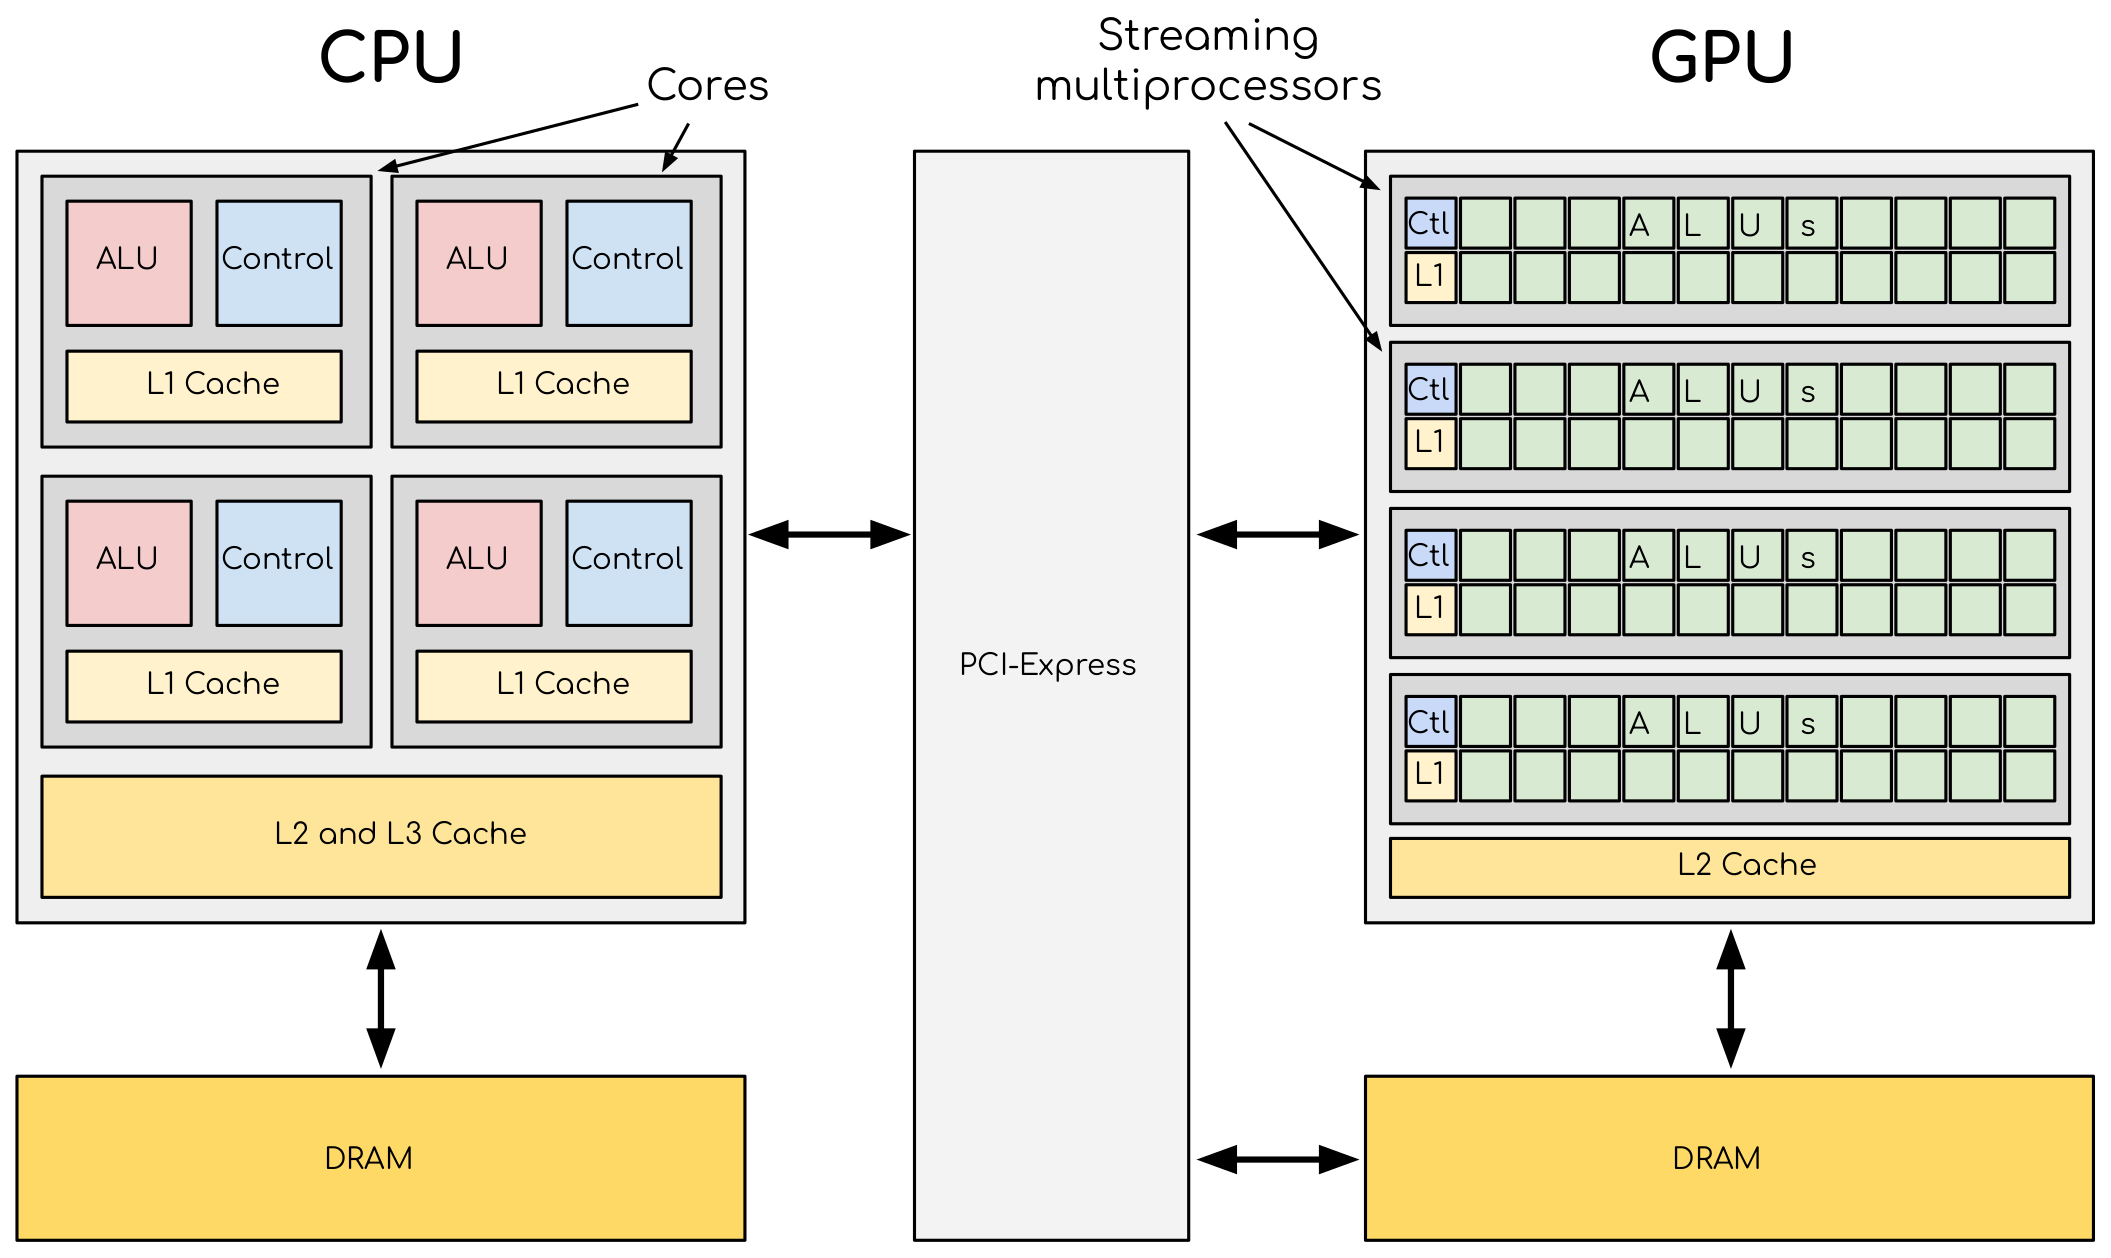
\includegraphics[width=\textwidth]{External Images/CPUandGPU.png}};
    \begin{scope}[x={(image.south east)}, y={(image.north west)}]
      \foreach \y in {0.806, 0.676, 0.545, 0.413} {
        \draw[fill=orange!80!black] (0.692,\y-0.047) rectangle (0.74,\y+0.035);
        \node[font=\sffamily\tiny, align=center, scale=0.9] at (0.716, \y-0.006) {Shared\\Memory};
      }
      \definecolor{maskYellow}{RGB}{254, 217, 102}
      \fill[maskYellow] (0.15,0.07) rectangle (0.164,0.092);
      \fill[maskYellow] (0.79,0.06) rectangle (0.802,0.10);
    \end{scope}
  \end{tikzpicture}
  \caption{Comparison of modern multi-core CPU and GPU architectures. The CPU features four cores, each containing an arithmetic logic unit (ALU) and control unit, supported by hierarchical cache memory (L1-L3) to minimize data transfer bottlenecks between the random access memory (RAM) and the cores. The GPU contains multiple streaming multiprocessors, each containing numerous processing units and shared memory for inter-thread communication, but minimal control logic. This architectural difference reflects their design priorities: CPUs optimize for sequential performance and complex control flow, while GPUs maximize parallel throughput. The PCI-Express serves as a communication interface between them. Adapted from material by ENCCS, licensed under \mbox{CC-BY 4.0 \cite{enccs2025gpu}.}}
  \label{fig:cpu-gpu-architecture}
\end{figure}

In contrast, while lacking the sophistication that makes CPUs excel at sequential and control-heavy tasks, GPUs dedicate most of their silicon area to processing units, creating massively parallel architectures optimized for numerical computation. GPU execution follows a \emph{single instruction multiple thread} (SIMT) paradigm: thousands of threads execute the same instruction in parallel \cite{cuda2025guide}. This increases throughput far beyond single- or multithreading on comparatively few CPU cores.

A modern GPU contains multiple independent \emph{streaming multiprocessors} (SMs), each comprising numerous processing units that share control logic and local memory resources \cite{kirk2016programming, cuda2025guide}. Within each multiprocessor, threads execute in groups of 32 called \emph{warps}. These warps generally operate in lockstep --- all threads in a warp execute the same instruction simultaneously on their respective data.\footnote{Since the NVIDIA Volta architecture (2017), threads within a warp can follow independent control paths, enabling more flexible algorithms. However, divergent execution reduces efficiency as different paths must be serialized \cite{cuda2025guide}.} Similarly to CPUs, all SMs share access to high-capacity but high-latency global memory (RAM), while each SM contains faster local caches. Additionally, each SM contains a programmer-managed memory region called \emph{shared memory}, enabling inter-thread communication within the same multiprocessor \cite{sanders2010cuda, cuda2025guide}.
\clearpage

\subsection{Parallel Computing Fundamentals}\label{subsec:parallell}

A theoretical framework helps to analyze parallelism opportunities and limitations. This section introduces key concepts for assessing algorithm structure, theoretical speedup limits, and common pitfalls.

Kirk and Hwu \cite{kirk2016programming} distinguish between two forms of parallelism: data parallelism and task parallelism. The former denotes performing the same operations in parallel on different data, while the latter means performing multiple different tasks simultaneously. An example of data parallelism is vector addition, where each respective component in vector A is added to its corresponding component in vector B. The authors argue that data parallelism is more abundant in modern computing as programs use increasingly large data sets. The SIMT-based architecture of GPUs is naturally highly optimized for data parallelism. This originates from graphics rendering, where identical operations must update many thousands of pixels simultaneously \cite{sanders2010cuda}.  While task parallelism is less suited to GPU architectures, it can still be exploited by partitioning programs into independent sub-tasks.

Acar \cite{acar2016parallel} provides a framework for formal analysis of parallel algorithms. Algorithms are represented as directed acyclic graphs (DAGs), where nodes represent executions of individual instructions and edges represent dependencies between them. The DAG can be viewed as a Hasse diagram that depicts a partial ordering of instructions under the relation "must execute before". Acar restricts the maximum node \emph{out-degree} and \emph{in-degree}\footnote{The number of edges extending out from or into a node.} to two, corresponding to spawning a new thread and synchronizing the result from two threads. \cref{fig:DAG-algo} depicts a DAG representation of an algorithm.

\begin{figure}[h]
\centering
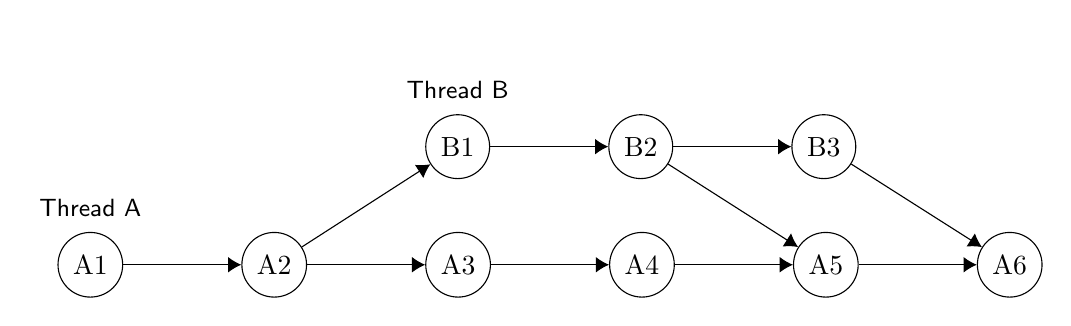
\begin{tikzpicture}[
    node distance=1.5cm and 1.5cm,
    every node/.style={draw, circle, minimum size=8mm},
    every edge/.style={draw, -{Latex[width=2mm]}},
    threadlabel/.style={font=\sffamily\small, draw=none, fill=none},
]
\node (A1) {A1};
\node[right=of A1] (A2) {A2};
\node[right=1.5cm and 1.5cm of A2, yshift=1.5cm] (B1) {B1};
\node[right=of A2] (A3) {A3};
\node[right=of B1] (B2) {B2};
\node[right=of A3] (A4) {A4};
\node[right=of A4] (A5) {A5};
\node[right=of B2] (B3) {B3};
\node[right=of A5] (A6) {A6};
\draw (A1) edge (A2);
\draw (A2) edge (B1);
\draw (A2) edge (A3);
\draw (B1) edge (B2);
\draw (A3) edge (A4);
\draw (A4) edge (A5);
\draw (B2) edge (A5);
\draw (B2) edge (B3);
\draw (A5) edge (A6);
\draw (B3) edge (A6);
\node[threadlabel, above=-0.5cm of B1] {Thread B};
\node[threadlabel, above=-0.5cm of A1] {Thread A};
\end{tikzpicture}
\caption{Directed acyclic graph (DAG) representation of a parallel algorithm. Nodes represent individual instructions and edges represent instruction dependencies that determine execution order. At node A2, a new thread is spawned, after which both threads execute independent instruction sequences in parallel. The threads synchronize at nodes A5 and A6, but thread B terminates only at the latter. DAG representations help visualize the algorithm structure and identify opportunities for parallel execution on independent paths.}
\label{fig:DAG-algo}
\end{figure}
\clearpage
Using these graphs, Acar \cite{acar2016parallel} defines the \emph{work} of an algorithm as the total number of nodes in the DAG, and \emph{span} as the length of its longest path. Alternatively, assuming each instruction takes a unit of time and no overhead cost of thread management, one can think of the work as the sequential run-time on a single processor $T_1$, and span as the run-time on an idealized infinite-processor machine $T_{\infty}$. For instance, the DAG presented in \cref{fig:DAG-algo} contains nine units of work but a span of only six units. It is now possible to define two lower bounds on algorithm run-time on a p-processor machine $T_p$:

\paragraph{Span-limited lower bound $T_p \geq T_\infty$ :} No matter the number of available processors, the execution cannot be faster than the longest dependency chain in the DAG. This illustrates the role of algorithm structure in parallelization potential, and motivates the effort to restructure algorithms to minimize span and other dependency chains.

\paragraph{Work-limited lower bound $T_p \geq T_1/p$ :} $p$ processors can perform at most $p$ operations in parallel, even if there are no dependencies. This highlights hardware constraints.

Furthermore, Acar demonstrates that for both level-by-level and \mbox{greedy scheduling}\footnote{Level-by-level scheduling assigns nodes to processors by a level-order traversal of the DAG. This can leave processors idle if the amount of nodes per level does not evenly divide the amount of processors. In contrast, greedy scheduling minimizes idle time by immediately assigning available nodes to idle processors.} the upper bound is within a factor 2 of the lower bound, again highlighting the importance of minimizing span and providing sufficient resources \cite{acar2016parallel}. In practice, runtime analysis is often more complex due to factors such as varying instruction latencies, parallelization overhead, and synchronization and shared resource contention.
\clearpage

\section{GPU Acceleration of the Cox-Ross-Rubinstein Binomial Model} \label{sec:gpu-crr}

\subsection{The Cox-Ross-Rubinstein Model}

The Cox-Ross-Rubinstein (CRR) model \cite{cox1979option} extends the single-period setting into its multi-period counterpart, providing a more realistic model of asset price evolution. The model maintains the same assumptions as before: discrete periods and constant multiplicative factors $u$ and $d$ for price movements. Over multiple periods, this creates a binomial lattice of possible price paths. This lattice expands outward from the initial stock price, generating a set of final states for the stock price and the corresponding option payoff.

The CRR model solves for the initial option value using backward induction. Starting at the terminal nodes, where option payoffs are calculated using \cref{eq:long_call_payoff,eq:long_put_payoff}, the algorithm works backward through the lattice. Each interior node is treated as a single-period problem, with option values calculated using \cref{eq:risk-neutral-expectancy}. \cref{fig:crr-twoperiod} visualizes a two-period lattice, though the model extends to any number of periods.

\begin{figure}[bp]
    \centering
    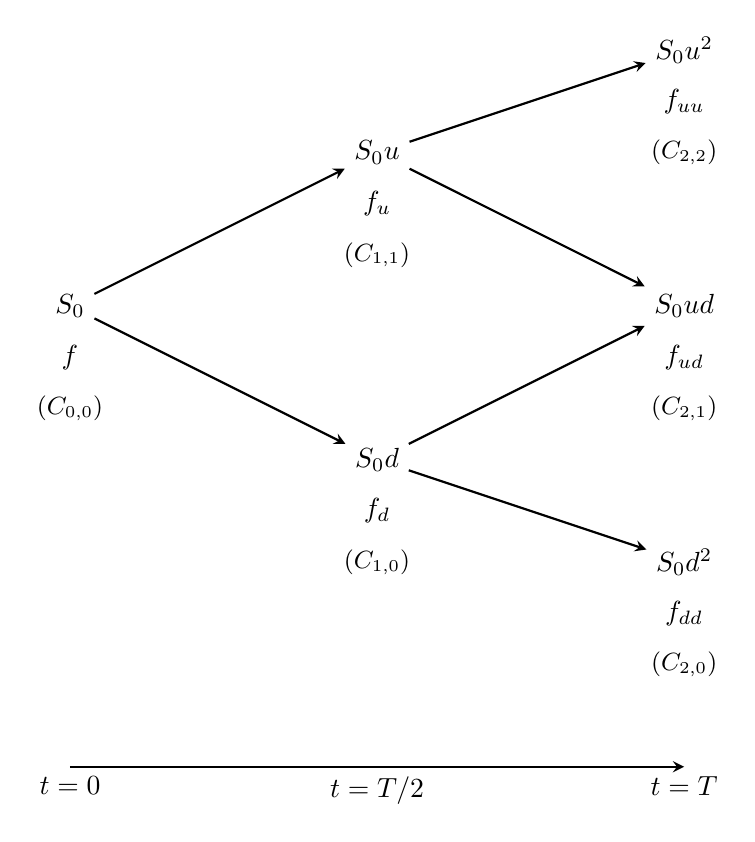
\begin{tikzpicture}[
        scale=1.3,
        >=stealth,
        every node/.style={font=\normalsize}
    ]
    \node (S0) at (0,0) {$S_0$};
    \node at (0,-0.5) {$f$};
    \node at (0,-1.0) {\small $(C_{0,0})$};
    \node (Su) at (3,1.5) {$S_0u$};
    \node at (3,1) {$f_u$};
    \node at (3,0.5) {\small $(C_{1,1})$};
    \node (Sd) at (3,-1.5) {$S_0d$};
    \node at (3,-2) {$f_d$};
    \node at (3,-2.5) {\small $(C_{1,0})$};
    \node (Suu) at (6,2.5) {$S_0u^2$};
    \node at (6,2) {$f_{uu}$};
    \node at (6,1.5) {\small $(C_{2,2})$};
    \node (Sud) at (6,0) {$S_0ud$};
    \node at (6,-0.5) {$f_{ud}$};
    \node at (6,-1.0) {\small $(C_{2,1})$};
    \node (Sdd) at (6,-2.5) {$S_0d^2$};
    \node at (6,-3) {$f_{dd}$};
    \node at (6,-3.5) {\small $(C_{2,0})$};
    \draw[->, thick] (S0) -- (Su);
    \draw[->, thick] (S0) -- (Sd);
    \draw[->, thick] (Su) -- (Suu);
    \draw[->, thick] (Su) -- (Sud);
    \draw[->, thick] (Sd) -- (Sud);
    \draw[->, thick] (Sd) -- (Sdd);
    \draw[->, thick] (0,-4.5) -- (6,-4.5);
    \node at (0,-4.5) [below] {$t=0$};
    \node at (3,-4.5) [below] {$t=T/2$};
    \node at (6,-4.5) [below] {$t=T$};
    \end{tikzpicture}
        \caption{Two-period binomial lattice. Stock prices evolve over time, creating an expanding set of possible outcomes. Option payoffs are calculated at the terminal nodes, after which option values at interior nodes can be calculated using \cref{eq:risk-neutral-expectancy}. The symbols $C_{i,j}$ represent the algorithmic notation for the option values, where $i$ indexes time and $j$ the number of up-ticks the stock price has moved.}
    \label{fig:crr-twoperiod}
\end{figure}
Cox, Ross, and Rubinstein defined $u = e^{\sigma\sqrt{T/n}}$ and $d = e^{-\sigma\sqrt{T/n}}$, where $\sigma$ is the annualized volatility of the asset's log-returns, $T$ is the total time in years, and $n$ is the number of periods \cite{cox1979option}. They show this to be useful for several reasons. First, it ensures the model converges to the famous Black-Scholes-Merton (BSM) model as $n \rightarrow \infty$. Second, the lattice recombines --- permutations of a price path reach the same node. This maintains computational feasibility as the number of states grows linearly with $n$ instead of exponentially. Additionally, the discount rate must be adjusted for $n$ such that it matches that of the one-period example. The continuous rate $e^{rT/n}$ is typically used instead of discrete compounding \cite{hull2013fundamentals}.

The following pseudocode is based on the implementation by Clewlow and Strickland \cite{clewlow1998implementing}. Let $S_0$ be the initial stock price and $n$ the number of periods. The nodes of the recombining lattice are indexed by $(i,j)$, where $0 \leq i \leq n$ indexes time\footnote{A period denotes an interval between two discrete points in time, hence for $n$ periods we have $n+1$ time points from $0$ to $n$.} and $0 \le j \le i$ the number of up-ticks $j$ the stock price has moved. The stock price at each node is defined as $S_{i,j} = S_0u^jd^{i-j}$, and $C_{i,j}$ denotes the corresponding option value. The option value  $C_{0,0}$ is calculated as shown in \cref{alg:crr-european}.

\begin{algorithm}
\LinesNumbered
\caption{CRR European Option Pricing}
\label{alg:crr-european}
\KwIn{$S_0$ (initial stock price), $K$ (strike price), $T$ (time to maturity), $r$ (risk-free rate), $n$ (periods), $\sigma$ (volatility), option type}
\KwOut{Option value at $t=0$}

$\Delta t \gets T/n$\;
$u \gets e^{\sigma\sqrt{\Delta t}}$\;
$d \gets 1/u$\;
$disc \gets e^{-r\Delta t}$\;
$p \gets (e^{r\Delta t} - d)/(u - d)$\;

\BlankLine
\tcp{Forward phase: compute stock prices at terminal nodes}
\For{$j \gets 0$ \KwTo $n$}{
    $S_j \gets S_0 \cdot u^j \cdot d^{n-j}$\;
}

\BlankLine
\tcp{Compute option payoffs at terminal nodes}
\For{$j \gets 0$ \KwTo $n$}{
    $C_j \gets \max(0, S_j - K)$ for call option\;
    $C_j \gets \max(0, K - S_j)$ for put option\;
}

\BlankLine
\tcp{Backward phase: compute option values through lattice}
\For{$i \gets n-1$ \KwSty{downto} $0$}{
    \For{$j \gets 0$ \KwTo $i$}{
        $C_j \gets disc \cdot (p \cdot C_{j+1} + (1-p) \cdot C_j)$\;
    }
}
 
\Return{$C_0$}\;
\end{algorithm}

The core of the algorithm lies in line 15, which directly implements the risk-neutral valuation principle shown in \cref{eq:risk-neutral-expectancy}. A key advantage of the CRR and other lattice-based models is their natural ability to price American options, which generally cannot be valued using closed-form solutions like the BSM model \cite{wilmott2013paul}. For American options, the option value calculation on line~15 is modified to include the early-exercise possibility:
\begin{equation*}
C[j] \gets \max(\text{payoff}(S[j]), disc \cdot (p \cdot C[j+1] + (1-p) \cdot C[j])),
\end{equation*}
where $\text{payoff}(S[j])$ equals $\max(K - S[j], 0)$ for puts or $\max(S[j] - K, 0)$ for calls, representing the immediate exercise value.

\subsection{Naive GPU-acceleration}
The sequential algorithm has asymptotic time complexity $O(n^2)$ due to the nested loop in the backward induction phase. This poses a significant computational challenge as the number of periods increases. While nodes at successive time points form a clear dependency chain, nodes at the same time point are independent and can be computed in parallel. This structure suggests substantial parallelization opportunities.

Kolb and Pharr \cite{pharr2005gpu} implement a GPU-accelerated version using this approach. At each time point, they spawn one thread per node, letting each thread compute a single node from its two child nodes. Threads synchronize after each time point to prevent data races. The implementation uses two alternating arrays for reading and writing intermediate results. To maximize GPU utilization, the algorithm is run in parallel for ``a thousand or so independent options''. The full source code is found in the original article\footnote{The implementation from 2005 predates CUDA, using the Cg language common for GPU programming at the time.}.

\begin{figure}[htbp]
    \centering
    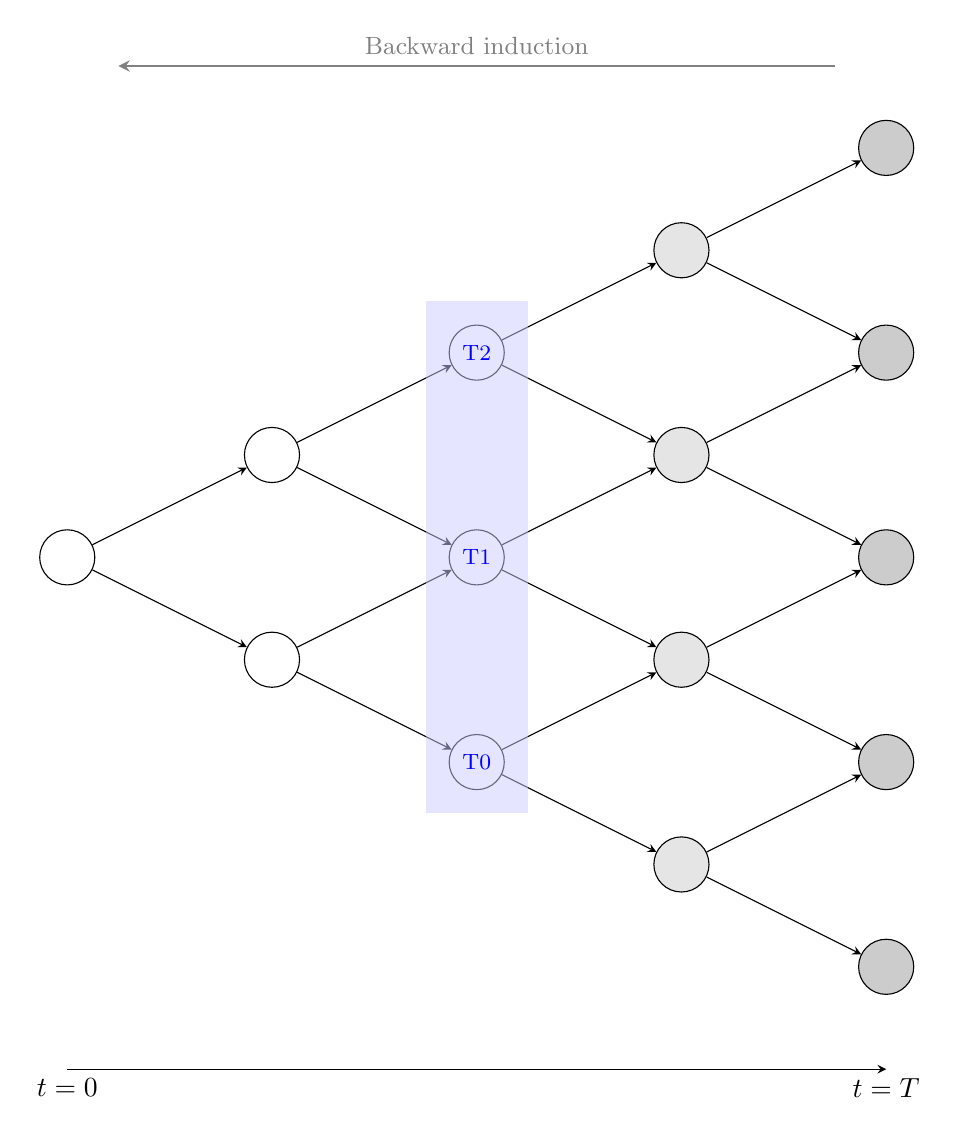
\begin{tikzpicture}[
        scale=1.3,
        >=stealth,
        every node/.style={font=\normalsize}
    ]
    
   % Draw lattice nodes
    \foreach \i in {0,...,4} {
        \foreach \j in {0,...,\i} {
            \pgfmathsetmacro\y{\j*2-\i}
            \ifnum\i=4
                \node[circle, draw, minimum size=7mm, fill=gray!40] (n\i\j) at (\i*2,\y) {};
            \else
                \ifnum\i=3
                    \node[circle, draw, minimum size=7mm, fill=gray!20] (n\i\j) at (\i*2,\y) {};
                \else
                    \node[circle, draw, minimum size=7mm] (n\i\j) at (\i*2,\y) {};
                \fi
            \fi
        }
    }
    
    \draw[<-, thick, gray] (0.5,4.8) -- (7.5,4.8);
    \node[gray] at (4,5) {\small Backward induction};
    
    % Draw edges
    \foreach \i in {0,...,3} {
        \pgfmathtruncatemacro\nexti{\i+1}
        \foreach \j in {0,...,\i} {
            \pgfmathtruncatemacro\nextj{\j+1}
            \draw[->] (n\i\j) -- (n\nexti\j);
            \draw[->] (n\i\j) -- (n\nexti\nextj);
        }
    }
    
    % Highlight one time column
    \fill[blue!20, opacity=0.5] (3.5,-2.5) rectangle (4.5,2.5);

    
    \node[blue, font=\footnotesize] at (4,-2) {T0};
    \node[blue, font=\footnotesize] at (4,0) {T1};
    \node[blue, font=\footnotesize] at (4,2) {T2};
    
    % Simple time labels
    \draw[->] (0,-5.0) -- (8,-5.0);
    \node at (0,-5.0) [below] {$t=0$};
    \node at (8,-5.0) [below] {$t=T$};
    
    \end{tikzpicture}
    \caption{Naive GPU acceleration of the Cox-Ross-Rubinstein (CRR) algorithm. The binomial lattice structure reveals instruction dependencies across time. Nodes at each time point can be computed in parallel by independent threads (T0, T1, T2) during backward induction. Filled nodes are already computed, with the terminal nodes in dark gray.}
    \label{fig:crr-gpu-naive}
\end{figure}

The parallel implementation does not redesign the algorithm in any way, but simply utilizes more resources for parallel computation. The work of the algorithm is thus $O(n^2)$, identical to the sequential time complexity. On the other hand, the span is only $O(n)$, so linear run-time is achievable with sufficient processors. \cref{fig:crr-gpu-naive} illustrates this parallel execution. Using $n=1024$ periods, the authors report throughput as a function of the number of American options processed. The single-threaded CPU implementation achieves approximately 110 options/s. The GPU version initially underperforms for batches of fewer than 5 options, likely due to parallelization overhead, but scales to approximately 1150 options/s with larger batches --- a 10x speedup. The throughput plateau suggests either full GPU utilization or other bottlenecks.

For large lattices, the naive parallelization encounters synchronization bottlenecks. Threads must synchronize after each time point, creating overhead that grows with $n$. This overhead is particularly severe when the lattice exceeds the capacity of a single streaming multiprocessor, forcing communication through slower global memory rather than shared memory. Suo et al. \cite{suo2015gpu} explore strategies to mitigate this. A naive attempt sacrifices parallelism by having a thread compute multiple nodes over several periods, thereby reducing synchronization frequency. This, however, leads to redundant computation as nodes at intermediate time points must be calculated multiple times by different threads. More sophisticated approaches avoid this redundancy --- the authors propose a ``triangle method'' that carefully partitions the lattice to minimize both synchronization overhead and redundant calculations.
\clearpage

\subsection{Additional Parallelization Across Time}
Ganesan et al. \cite{ganesan2009acceleration} present another approach that exploits parallelism across time, not just at individual time points. This is achieved by a reformulation of the problem that establishes direct relationships between non-adjacent nodes. \cref{eq:risk-neutral-expectancy} relates the option values at time $i$ to the values at time $i+1$. By repeatedly substituting this formula into itself and expanding, one obtains a general relationship between option values at time $i-m$ and those at time $i$:

\begin{equation}
    F_{i-m}(j) = e^{-m r \Delta t} \sum_{k=0}^m c_k F_i(j+k)
\label{eq:relative-prices}
\end{equation}
where $j$ indexes the nodes at time $i-m$, and the coefficients $c_k, 0 \leq k \leq m$ represent the (risk-neutral) probabilities of all paths from node $(i-m,j)$ to node $(i,j+k)$. These are simply binomial coefficients weighted by the appropriate powers of the probabilities: $c_k = \binom{m}{k}p^k(1-p)^{m-k}$. The key insight is that while the coefficients in this reformulation still exhibit the same sequential dependencies between successive time points, they can be computed independently for different segments of the lattice. Unlike the actual option values, there is no strict requirement for starting at the terminal nodes when calculating these coefficients.

Based on this insight, the authors present the following parallel algorithm \cite{ganesan2009acceleration}: First, divide the $n$-period lattice into $p$ partitions of length $n/p$. Each partition then computes coefficients relating the nodes at its left boundary to the ones at its right boundary. These independent operations proceed in parallel across all partitions. Once the coefficients are computed, the option values can be propagated from right to left across partition boundaries using \cref{eq:relative-prices}. This requires only $p$ sequential steps rather than $n$ \footnote{While the authors claim this method extends to American options, they provide insufficient detail on how early exercise opportunities are evaluated when intermediate nodes are computed after the main propagation phase.}. \cref{fig:partitioned} illustrates the idea.

\begin{figure}[h]
    \centering
    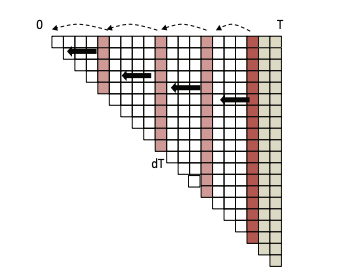
\includegraphics[scale=0.6]{External Images/CRRpartitioned.png}
    \caption{Partitioned Cox-Ross-Rubinstein (CRR) algorithm for parallel computation across time. The binomial lattice is divided into partitions. Within each partition, coefficients relating nodes at left and right boundaries are computed in parallel. Once coefficients are computed, option values propagate sequentially from right to left across partition boundaries, skipping many intermediate values. The rightmost partition can alternatively compute option values directly using standard backward induction, as is done in the figure. Reproduced with permission from the authors \cite{ganesan2009acceleration}.}

    \label{fig:partitioned}
\end{figure}

The total work remains $O(n^2)$ since every node must still be processed, either directly calculating the option value or the corresponding coefficient. The span, however, is further reduced from $O(n)$ to $O(n/p + p)$ due to the algorithmic reformulation. The corresponding DAG transforms from a tall, narrow lattice into a shorter, wider one. In the GPU implementation, partitions are computed on independent streaming multiprocessors. Communication between partitions is done through global memory, introducing latency $L$ at each propagation step \cite{ganesan2009acceleration}. Increasing $p$ improves execution time up to a certain point, where the communication latency and boundary calculation overhead outweighs the benefit of additional parallelism. The authors derive the optimal number of partitions as $p = \sqrt{2n/L}$ \cite{ganesan2009acceleration}. In practice, they achieve a 2x speedup over a naive GPU implementation. In clear contrast to bulk pricing, this approach dedicates all computing resources to an individual option, making it suitable for pricing of a single or small group of key portfolio assets.

\section{GPU Acceleration of Monte Carlo Methods} \label{sec:gpu-mc}
\subsection{Monte Carlo Methods}
Monte Carlo (MC) methods are a class of computational algorithms that approximate solutions to problems through random sampling. Unlike analytical solutions and deterministic numerical methods, both of which rely on domain-specific mathematical theory, MC methods are relatively simple and broadly applicable across many domains. The theoretical foundation is the \emph{law of large numbers}, which states that the sample average tends toward the true expected value with increasing sample size \cite{Ross2020prob}. Therefore, with a well-chosen sampling distribution whose expectation matches the target quantity, the average of a large number of simulated outcomes provides a reliable approximation of the solution.

While true random number generation is difficult, there exist many so-called pseudorandom number generators (RNGs) whose deterministic sequences are statistically indistinguishable from true randomness. Most RNGs first generate samples from a uniform distribution $U(0,1)$, and then apply a transformation to map these to the desired distribution. The Box-Muller transform, for instance, converts uniform samples to normally distributed values: $U(0,1) \rightarrow N(0,1)$ \cite{gentle2003random}.

Many software libraries provide RNGs for various distributions. Combined with affordable computing power, this has driven widespread adoption of MC methods across different domains. However, their generality comes at a significant computational cost. While analytical and deterministic methods exploit problem-specific structure for faster convergence, MC methods typically require many iterations to achieve accuracy. Nevertheless, MC methods excel at high-dimensional problems where traditional approaches fail or become exceedingly slow \cite{gentle2003random}. In derivatives pricing, MC methods are mostly used for exotic options with complex payoff structures, for example basket options whose payoffs depend on numerous underlying assets \cite{hull2016options,wilmott2013paul}.

MC option pricing relies on the same risk-neutral valuation framework presented in \cref{sec:risk-neutral-theory}. While the BSM model solves a partial differential equation analytically for the expected discounted payoff, the MC approach estimates this value by averaging many simulated option payoffs, each computed from a risk-neutral stock price path \cite{boyle1977options}. This estimate converges toward the theoretical value as the number of simulations increases.

MC simulation typically models stock price dynamics using a discretized version of the \emph{geometric Brownian motion} process used in the BSM model. This is also the stock price dynamics of the CRR model in the limit as $n \rightarrow \infty$ \cite{cox1979option}. Under these assumptions, one can solve for the exact distribution of the stock price at any future time point, and thus the discretization does not introduce an error \cite{clewlow1998implementing}. After each period, the stock price is updated according to
\begin{equation*}
S_{t+\Delta t} = S_t \cdot \exp \left( \nu \Delta t + \sigma \sqrt{\Delta t} \cdot \epsilon_i \right),
\label{eq:GBM-price}
\end{equation*}
where $\nu=r-\frac{1}{2}\sigma^2$ is a deterministic growth component and $\epsilon_i \sim N(0,1)$ is a standard normal variable for random price fluctuations \cite{clewlow1998implementing}. Hence, there is no need to use more than one period unless the payoff is path dependent. Asian options, for example, have payoffs based on mean stock prices over the holding period. In this case, much like the CRR model, we get a better approximation with a smaller time step. \cref{alg:MC-algo}, based on Clewlow and Strickland \cite{clewlow1998implementing}, demonstrates a generic implementation of MC option pricing. Simulating $m$ paths of length $n$ and evaluating a payoff with cost $p$ yields a time complexity of $O(m \cdot (n+p))$. For most payoffs $p=O(1)$ as even path-dependent payoffs can often be computed incrementally during path generation. For European options where $n=1$, this reduces to $O(m)$.

\begin{algorithm}
\LinesNumbered
\caption{MC Option Pricing}
\label{alg:MC-algo}
\KwIn{$S_0$ (initial stock price), $K$ (strike price), $T$ (time to maturity), $r$ (risk-free rate), $n$ (periods), $\sigma$ (volatility), $M$ (paths), option type, payoff function}
\KwOut{Option value at $t=0$}

$\Delta t \gets T/n$\;
$\nu \gets r - 0.5 \cdot \sigma^2$\;
$\text{nudt} \gets \nu \cdot \Delta t$\;
$\text{sigsqrt} \gets \sigma \cdot \sqrt{\Delta t}$\;
$C_{\text{sum}} \gets 0$\;

\BlankLine
\tcp{Simulate $M$ stock price paths}
\For{$m \gets 1$ \KwTo $M$}{
    $S[0] \gets S_0$\;
    \BlankLine
    \tcp{Generate price path over $n$ periods}
    \For{$i \gets 1$ \KwTo $n$}{
        Sample $\epsilon \sim \mathcal{N}(0,1)$\;
        $\ln S[i] \gets \ln S[i-1] + \text{nudt} + \text{sigsqrt} \cdot \epsilon$\;
        $S[i] \gets \exp(\ln S[i])$\;
    }
    \BlankLine
    \tcp{Compute payoff for this path}
    $C_m \gets \text{payoff}(S[0..n], K)$\;
    $C_{\text{sum}} \gets C_{\text{sum}} + C_m$\;
}

\BlankLine
\tcp{Average and discount payoffs}
$C_0 \gets e^{-rT} \cdot \frac{C_{\text{sum}}}{M}$\;

\Return{$C_0$}\;
\end{algorithm}


\subsection{Naive GPU-acceleration}
MC simulation is considered an \emph{embarrassingly parallel} problem --- each path is independent, allowing straightforward parallelization without further redesign. By a similar argument as earlier, the work of the algorithm therefore equals the sequential time complexity $O(m \cdot (n+p))$. The span is $O(n+p)$, assuming an infinite-processor machine that can simulate all $m$ paths in parallel.

Instead, the primary challenge becomes generating independent random numbers across threads. Naive parallelization can produce correlated number sequences between threads, violating the independence assumption of MC simulation. Effective implementations must therefore partition the RNG state space to ensure statistical independence across all threads \cite{gentle2003random}. Early GPU implementations, like the one by Howes and Thomas \cite{nguyen2007gpu}, had to manually construct such generators. Today, GPU libraries like cuRAND \cite{curand2025} provide parallel RNGs as standard functionality, eliminating the need for manual implementation.

Howes and Thomas \cite{nguyen2007gpu} benchmarked GPU-accelerated MC option pricing using an Nvidia GeForce 8 GPU and quad-core AMD Opteron 2.2 GHz CPU. They achieved a 26x speedup for random number generation alone, with overall speedups of 59x for Asian options and 23x for a variant of lookback options. These results show that even fairly naive GPU implementations of the early days (2007) achieved substantial speedups over multi-core CPU versions, despite the inherent challenges of parallel random number generation. When isolating the simulation-related computations (using constants instead of random numbers), speedups reached 118x and 45x respectively. This indicates that random number generation becomes the dominant bottleneck in GPU implementations. 

The choice of random number generator often depends on the option type and memory constraints, as some option payoffs require storing intermediate values in memory. In this example, the sum used for the mean calculation in the Asian option can be accumulated in a single variable, leading to minimal memory requirements. This enabled the use of the faster Wallace RNG, which could not be used in the pricing of more memory-intensive variant of lookback options that needed to store entire price paths.

\subsection{Further Hardware Optimization}
Unlike the CRR algorithm, where reformulation was necessary to expose hidden parallelism, MC simulation presents a fundamentally different optimization challenge. The parallelism is already fully exposed at the algorithmic level --- each simulation path is completely independent, requiring no communication or synchronization with other paths. This embarrassingly parallel structure means that further speedups must instead come from efficiently mapping this parallelism onto GPU hardware. While variance reduction techniques and the use of quasi-random numbers can improve convergence rates \cite{clewlow1998implementing}, they benefit all implementations equally and are thus not relevant. Instead, GPU-specific optimizations focus on mitigating hardware constraints: efficient random number generation, memory access patterns and resource utilization. 

Liu et al.\ \cite{liu2010efficient} demonstrate several hardware-specific optimizations for GPU-accelerated MC option pricing, focusing on memory access inefficiencies and resource underutilization. The first optimization was to compress the working set, that is the amount of memory each thread must keep track of during simulation, to minimize expensive global memory access. The extent to which this is achievable heavily depends on the option type and choice of RNG. Memory bandwidth bottlenecks are addressed through coalesced access patterns, where adjacent threads access contiguous memory locations that can be fetched simultaneously. Register pressure presents another challenge. GPUs have limited registers per streaming multiprocessor, so implementations requiring many registers per thread reduce the number of concurrent threads. The authors propose splitting the work into smaller GPU kernels\footnote{A GPU kernel is a function executed in parallel by many threads} responsible for separate sub-tasks. While this reduces register pressure, it comes at a cost of additional global memory transfers between kernels. Together, these optimizations achieved a 43x speedup for exotic option pricing on an Nvidia Tesla C1060 GPU compared to an Intel 8-core Xeon 2.0 GHz CPU.

The authors also examine two different execution strategies for large workloads, where a single thread computes multiple stock price paths. In ``path mode'', the thread computes its assigned paths sequentially from start to finish. This minimizes memory usage and suits homogeneous workloads, like simulating paths for the same option. In ``slice mode'', the thread instead simulates one step at a time for all its price paths. This is more memory intensive as intermediary data is stored for all the paths. On the other hand, slice mode handles heterogeneous workloads better, for example simultaneous pricing of different options. If these options have different maturities, some path simulations will finish earlier than others, leading to warp divergence \cite{liu2010efficient}. Slice mode organizes the computations to minimize the associated overhead cost. \cref{fig:gpu-divergence} depicts the different execution modes and their effect on divergence. While GPU architectures have evolved significantly since the paper was published in 2010, the underlying tradeoffs between memory usage and thread utilization remain central to high-performance MC implementations.

\begin{figure}[htbp]
\centering
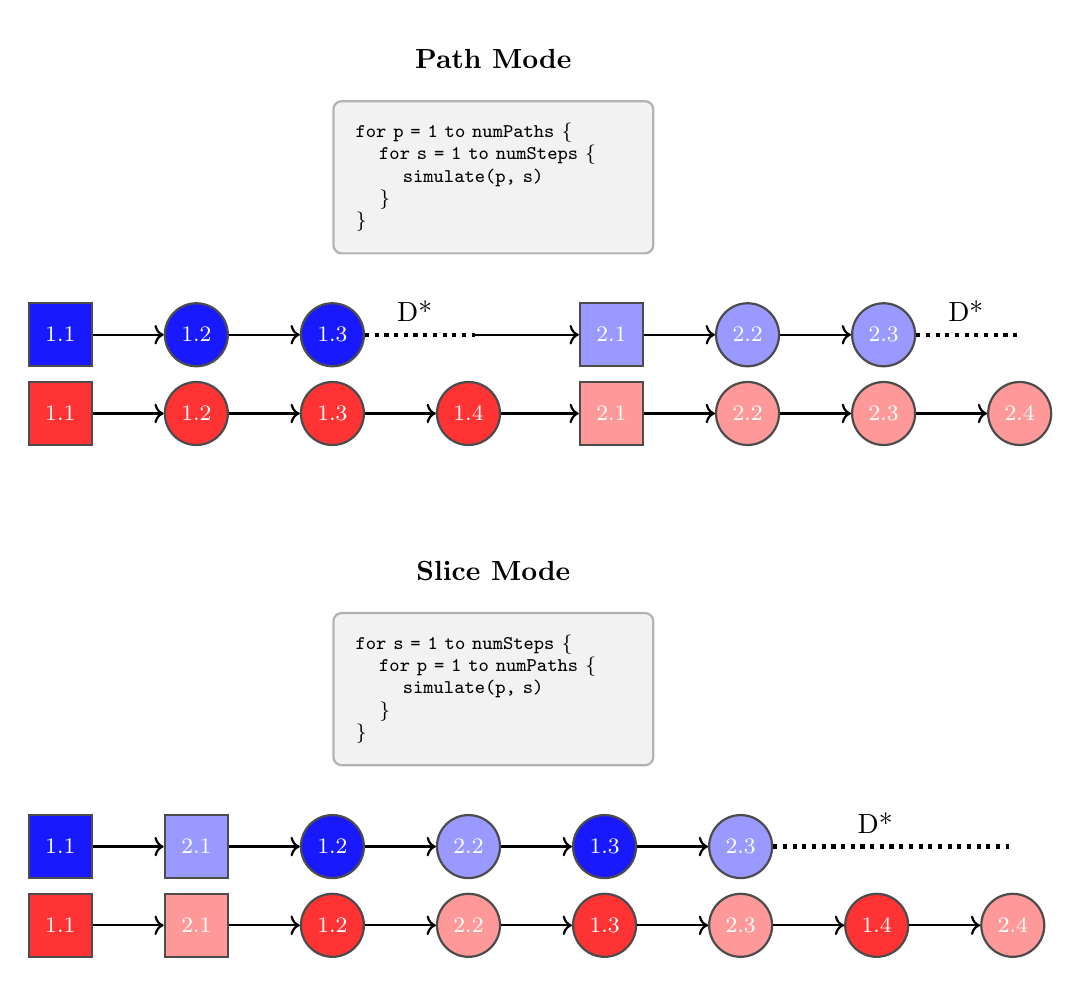
\begin{tikzpicture}[
    node distance=0.9cm,
    every node/.style={minimum size=0.8cm, font=\footnotesize, thick, draw=black!70, inner sep=0pt}
]

% Calculate center position
\def\centerx{6}

% Path Mode Title
\node[draw=none, font=\bfseries] at (\centerx, 9.5) {Path Mode};

% Path Mode Pseudocode
\node[draw=black!30, fill=gray!10, text width=3.5cm, align=left, font=\ttfamily\scriptsize, inner sep=8pt, rounded corners=3pt] at (\centerx, 8) {
for p = 1 to numPaths \{\\
\hspace{0.3cm}for s = 1 to numSteps \{\\
\hspace{0.6cm}simulate(p, s)\\
\hspace{0.3cm}\}\\
\}
};

% PATH MODE
% Thread 1 (Blue) - Path 1
\node[rectangle, fill=blue!90, text=white] (b11) at (0.5, 6) {1.1};
\node[circle, fill=blue!90, text=white, right=of b11] (b12) {1.2};
\node[circle, fill=blue!90, text=white, right=of b12] (b13) {1.3};

% Thread 2 (Red) - Path 1  
\node[rectangle, fill=red!80, text=white] (g11) at (0.5, 5) {1.1};
\node[circle, fill=red!80, text=white, right=of g11] (g12) {1.2};
\node[circle, fill=red!80, text=white, right=of g12] (g13) {1.3};
\node[circle, fill=red!80, text=white, right=of g13] (g14) {1.4};

% Dotted line and DIVERGENCE text after path 1
\draw[dotted, line width=1.5pt] (b13.east) -- ++(1.4,0) coordinate (b_dotted_end);
\node[draw=none, font=\normalsize] at (5, 6.3) {D*};

% Thread 1 (Blue) - Path 2 (lighter)
\node[rectangle, fill=blue!40, text=white] (b21) at (7.5, 6) {2.1};
\node[circle, fill=blue!40, text=white, right=of b21] (b22) {2.2};
\node[circle, fill=blue!40, text=white, right=of b22] (b23) {2.3};

% Thread 2 (Red) - Path 2 (lighter)
\node[rectangle, fill=red!40, text=white] (g21) at (7.5, 5) {2.1};
\node[circle, fill=red!40, text=white, right=of g21] (g22) {2.2};
\node[circle, fill=red!40, text=white, right=of g22] (g23) {2.3};
\node[circle, fill=red!40, text=white, right=of g23] (g24) {2.4};

% Dotted line and DIVERGENCE text after path 2
\draw[dotted, line width=1.5pt] (b23.east) -- ++(1.3,0);
\node[draw=none, font=\normalsize] at (12, 6.3) {D*};

% Arrows
\foreach \i/\j in {b11/b12, b12/b13, g11/g12, g12/g13, g13/g14,
                   b21/b22, b22/b23, g21/g22, g22/g23, g23/g24}
    \draw[->, thick] (\i) -- (\j);

% New arrows from path 1 to path 2
\draw[->, thick] (g14) -- (g21);
\draw[->, thick] (b_dotted_end) -- (b21);

% SLICE MODE
\node[draw=none, font=\bfseries] at (\centerx, 3) {Slice Mode};

% Slice Mode Pseudocode  
\node[draw=black!30, fill=gray!10, text width=3.5cm, align=left, font=\ttfamily\scriptsize, inner sep=8pt, rounded corners=3pt] at (\centerx, 1.5) {
for s = 1 to numSteps \{\\
\hspace{0.3cm}for p = 1 to numPaths \{\\
\hspace{0.6cm}simulate(p, s)\\
\hspace{0.3cm}\}\\
\}
};

% Thread 1 (Blue) - alternating colors
\node[rectangle, fill=blue!90, text=white] (sb11) at (0.5, -0.5) {1.1};
\node[rectangle, fill=blue!40, text=white, right=of sb11] (sb21) {2.1};
\node[circle, fill=blue!90, text=white, right=of sb21] (sb12) {1.2};
\node[circle, fill=blue!40, text=white, right=of sb12] (sb22) {2.2};
\node[circle, fill=blue!90, text=white, right=of sb22] (sb13) {1.3};
\node[circle, fill=blue!40, text=white, right=of sb13] (sb23) {2.3};

% Thread 2 (Red) - alternating colors
\node[rectangle, fill=red!80, text=white] (sg11) at (0.5, -1.5) {1.1};
\node[rectangle, fill=red!40, text=white, right=of sg11] (sg21) {2.1};
\node[circle, fill=red!80, text=white, right=of sg21] (sg12) {1.2};
\node[circle, fill=red!40, text=white, right=of sg12] (sg22) {2.2};
\node[circle, fill=red!80, text=white, right=of sg22] (sg13) {1.3};
\node[circle, fill=red!40, text=white, right=of sg13] (sg23) {2.3};
\node[circle, fill=red!80, text=white, right=of sg23] (sg14) {1.4};
\node[circle, fill=red!40, text=white, right=of sg14] (sg24) {2.4};

% Arrows
\foreach \i/\j in {sb11/sb21, sb21/sb12, sb12/sb22, sb22/sb13, sb13/sb23,
                   sg11/sg21, sg21/sg12, sg12/sg22, sg22/sg13, sg13/sg23,
                   sg23/sg14, sg14/sg24}
    \draw[->, thick] (\i) -- (\j);

% Single divergence - dotted horizontal line
\draw[dotted, line width=1.5pt] (sb23.east) -- ++(3,0);
\node[draw=none, font=\normalsize] at (10.85, -0.2) {D*};

\end{tikzpicture}
\caption{GPU warp divergence under heterogeneous workloads in ``path'' versus ``slice'' execution modes, as described by Liu et al. \cite{liu2010efficient}. Nodes representing simulation steps are labeled $(p,s)$ where $p$ is the path index and $s$ is the step index. $D^*$ denotes warp divergence. In path mode, threads complete entire paths sequentially, causing divergence when the paths differ in length. In slice mode, threads execute the same step across all paths before proceeding, resulting in a single divergence section at the end of the workload. While total idle time is theoretically the same, path mode's multiple divergence sections create more overhead, making slice mode more efficient for heterogeneous workloads. }

\label{fig:gpu-divergence}
\end{figure}

\section{Summary and Conclusions}  \label{sec:summary-conclusions}
This thesis evaluates the effectiveness of GPU acceleration for two widely used option pricing approaches: The Cox-Ross-Rubinstein (CRR) algorithm and Monte Carlo (MC) simulation. The analysis examines their parallelization potential, implementation strategies, achievable speedups and performance bottlenecks. The data show that both algorithms benefit significantly from GPU acceleration, though their inherent characteristics dictate different optimization approaches and performance gains. The results of the reviewed research are aggregated in \cref{tab:results-table}.

The algorithms' structures explain their initial GPU performance. The CRR model's backward induction creates dependencies across time points, limiting parallelization to computations within each time point. By contrast, MC simulation computes independent stock price paths, making it ideally suited for parallel execution. While direct comparison is complicated by differences in GPU hardware, the reported results are consistent with this distinction: the naive CRR-GPU implementation achieved an approximately 10x speedup over a single-core CPU \cite{pharr2005gpu}, whereas the MC-GPU implementation reported 23-59x speedups despite being benchmarked against a quad-core CPU \cite{nguyen2007gpu}. The disparity can likely be attributed to synchronization overhead affecting the CRR algorithm. Nonetheless, both naive implementations yield substantial improvements relative to implementation effort, making GPU acceleration worthwhile for either algorithm. 

Given these characteristics, further optimization strategies take different forms. The CRR model benefits from algorithmic reformulation to expose hidden parallelism, as demonstrated by Ganesan et al. \cite{ganesan2009acceleration} who partitioned the time axis to achieve a 2x improvement over a naive GPU implementation. MC methods already expose the available parallelism, and benefit more from hardware-specific optimizations. Liu et al. \cite{liu2010efficient} achieved a 43x speedup over a CPU baseline through techniques including memory coalescing and minimizing warp divergence. Ultimately, both algorithms face scalability limits: CRR implementations contend with synchronization or communication overhead, while MC simulation remains constrained by memory bandwidth, particularly when using memory-intensive random number generators.

While the results suggest MC methods may achieve larger GPU speedups, this does not make them the optimal solution for option pricing. In practice, the choice of algorithm depends on multiple factors: option type, available hardware, and other case-specific requirements and constraints. For instance, vanilla options are rarely priced using MC methods since analytical or lattice-based models often provide faster solutions. The practical approach is to first select an appropriate pricing model and then apply GPU acceleration. This becomes particularly valuable for high-throughput applications like portfolio-wide risk calculations or bulk pricing operations.

An important caveat is that the analyzed research spans 2005-2010. Cutting-edge research often remains proprietary within financial institutions that safeguard their competitive advantage, making it difficult to review the most recent developments in the field. GPU architectures have also evolved dramatically since then, largely driven by the massive demand for AI computing. Modern GPUs feature improved memory hierarchies, better divergence handling, and enhanced support for general-purpose computing, mitigating several of the mentioned bottlenecks while perhaps introducing new ones. Likewise, modern multi-core CPUs provide faster baselines than those in the original studies. Despite these hardware advances, the fundamental principle persists: effective GPU utilization requires both clever algorithmic design and hardware-conscious optimization. Future work could benchmark these algorithms on current architectures to enable direct comparisons. Additional research opportunities include GPU acceleration of other models, such as finite difference or machine learning-based methods.

\begin{table}[h]
\centering
\begin{threeparttable}
\caption{Empirically measured GPU speedups for selected option pricing models. Reported results are based on real implementations with varying baseline architecture and research methodologies. While not directly comparable, they provide indicative insight into performance improvements when interpreted with appropriate caution.}


\label{tab:results-table}
\begin{tabular}{lrp{4.5cm}p{4.5cm}}
\toprule
\textbf{Algorithm} & \textbf{\shortstack{Reported\\Speedup}} & \textbf{Strategy} & \textbf{Bottleneck} \\
\midrule
CRR\\
\cmidrule{1-2}
Naive & 10x\tnote{1} & Parallelization within time points & Synchronization latency between time points \\
Partitioned & 2x\tnote{2} & Additional parallelization across time periods & Inter-partition communication \\
\addlinespace 
MC\\
\cmidrule{1-2}
Naive & 23–59x\tnote{3} & Parallel simulation paths & random number generation, memory bandwidth \\
Optimized & 43x\tnote{4} & Memory coalescing, register reuse, warp divergence minimization & Memory bandwidth and register pressure \\
\bottomrule
\end{tabular}
\begin{tablenotes}
\footnotesize
\item[1] NVIDIA GeForce 6800 Ultra vs single-core 2.0GHz CPU (2005). \cite{pharr2005gpu}
\item[2] NVIDIA Tesla C1060 vs CRR Naive on the same architecture (2009) \cite{ganesan2009acceleration}.
\item[3] NVIDIA GeForce 8800 vs 4-core 2.2GHz CPU (2007). \cite{nguyen2007gpu}
\item[4] NVIDIA Tesla C1060 vs 8-core 2.0GHz CPU (2010). \cite{liu2010efficient}
\end{tablenotes}
\end{threeparttable}
\end{table}

\cleardoublepage

% Start of Appendices
\appendix
\section{Derivation of Risk-Neutral Probability Form}  % For 
\label{appendix:risk_neutral_derivation}

In this appendix, we derive the risk-neutral probability form of the one-period binomial model option pricing formula.

\begin{align}
&\text{Starting from \eqref{eq:replicating-portfolio}:} \nonumber\\[0.7em]
&\frac{f_u - f_d}{S_0(u-d)}S_0 + \frac{f_d \cdot u-f_u \cdot d}{(u-d)(1+r)} \nonumber\\[0.7em]
&=\frac{f_u - f_d}{u-d} + \frac{f_d \cdot u-f_u \cdot d}{(u-d)(1+r)} \nonumber\\[0.7em]
&=\frac{(f_u - f_d)(1+r)}{(u-d)(1+r)} + \frac{f_d \cdot u - f_u \cdot d}{(u-d)(1+r)} \nonumber\\[0.7em]
&=\frac{f_u(1+r) - f_d(1+r) + f_d \cdot u - f_u \cdot d}{(u-d)(1+r)} \nonumber\\[0.7em]
&= \frac{f_u[(1+r) - d] + f_d[u - (1+r)]}{(u-d)(1+r)} \nonumber\\[0.7em]
&= \frac{1}{1+r} \cdot \frac{f_u[(1+r) - d] + f_d[u - (1+r)]}{u-d} \nonumber\\[0.7em]
&= \frac{1}{1+r} \left( f_u \cdot \frac{(1+r) - d}{u-d} + f_d \cdot \frac{u - (1+r)}{u-d} \right)\nonumber
\end{align}

This final form reveals the risk-neutral probabilities: $\tilde p = \frac{(1+r) - d}{u-d}$ and $\tilde q = 1-\tilde p = \frac{u - (1+r)}{u-d}$.

The no-arbitrage condition ensures $\tilde p$ and $\tilde q$ are correctly bounded by 0 and 1. If $1+r > u$, investors could profit by shorting the stock and investing in the risk-free asset. Conversely, if $d > 1+r$, they could earn guaranteed profits. Therefore, $d \leq 1+r \leq u$ must hold, which leads to $0\leq \tilde p, \tilde q \leq 1$. Furthermore, $\tilde p + \tilde q = 1$. Thus, our risk-neutral probabilities form a valid probability distribution over the two possible outcomes.





\phantomsection

\addcontentsline{toc}{chapter}{\bibname}
\bibliographystyle{IEEEtran}
\bibliography{bibliography.bib}


\end{document}